\setstretchnormal

\chapter{Model Development}
\label{sect:modelling}

% Textbox
\begin{center}
	\begin{tcolorbox}[title=\boxtitle]
		\begin{itemize}[leftmargin=*,labelindent=2ex,labelsep=1.5ex,itemsep=0pt,parsep=0pt]
			\item How should the bioelectric models be created?
			\item What are the required inputs?
			\item What specific steps were followed to create the models?
		\end{itemize}
	\end{tcolorbox}
\end{center}

% This chapter documents how the models in this thesis were created. It begins
% with a preliminary discussion on the available \textit{in silico} numerical
% methods and the rationale for choosing the finite element method. This is
% followed by a survey of the required inputs, and a workflow for combining all of
% these inputs into a virtual representation of the implanted cochlea. An initial
% proof of concept workflow was evolved into a more robust version that was then
% implemented on two volumetric datasets: a guinea pig cochlea from a stack of
% sTSLIM images, and a human cochlea from a stack of microCT images. These models
% are then used for the investigations detailed in chapters 5--7.

%% ========================================================== Modelling Approach

\section{Introduction}

The overarching goal of this thesis is to determine how volume conduction models
(VCMs) of the cochlea can be improved. An accurate VCM would allow a better
spatial understanding of the cochlear implant (CI) system to be obtained, and
for the research questions detailed in \S\ref{sect:research_questions} to be
answered. To achieve these outcomes, it was important to develop and implement a
methodology that was robust, flexible, and efficient, which was not a trivial
task given the challenges in model
creation~\cite{briaire2000mesh,whiten2007,potratz2010,saba2012}. Therefore, a
number of solution methods, software packages, and input parameters were
critically considered. The initial workflow was progressively evolved to
overcome a number of different computational issues, and to represent the data
more intuitively so that implications could be inferred and conclusions easily
drawn.

This chapter documents the groundwork required to prepare the models of the
thesis for more in depth simulation studies. It covers the foundational work
that was performed to get the models into COMSOL, such as the imaging,
reconstruction and discretisation of the spatial domain, and consideration of
other required inputs such as material properties, loading, and boundary
conditions. The extensive documentation is intended to provide some guidance for
others looking to undertake development of a cochlear VCM. Details of the actual
analyses, including simulation results, are provided in the subsequent chapters.

\section{Preliminary Considerations}

\subsection{Modelling Workflow}

\subsubsection{Generalised Pipeline}

The typical flow of data when creating a VCM has been summarised by both
MacLeod~\cite{macleod2009} and Lau~\cite{lau2011}. The model development
workflow used for this project was informed by these procedures and is
illustrated in Figure~\ref{fig:workflow_general}.

\begin{figure}
	\centering
	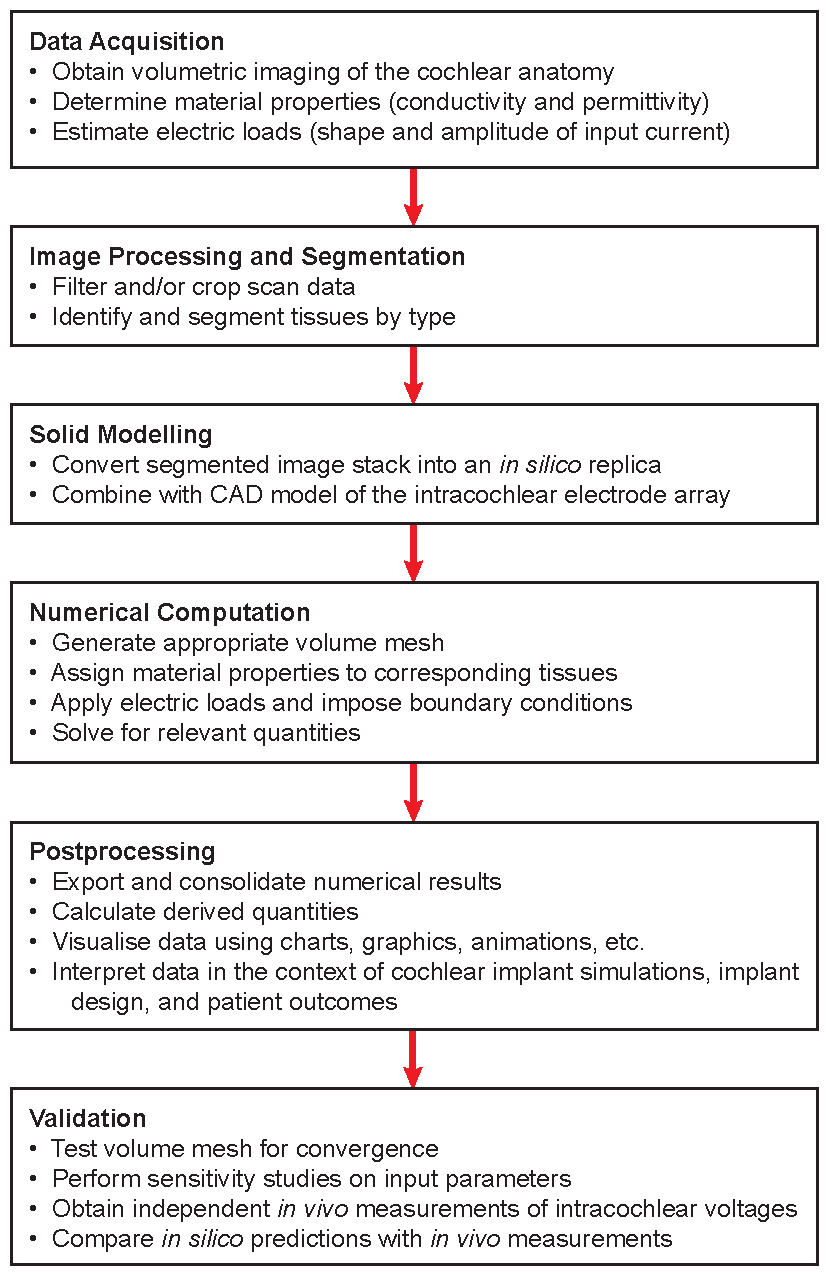
\includegraphics[width=11.8cm]{Methodology/workflow_general}
	\caption[Overview workflow schematic]{Overview workflow schematic, summarising
	the key objectives of each stage and the flow of data along the pipeline.}
	\label{fig:workflow_general}
\end{figure}

The first stage of the workflow is creating the model geometry, and there are
two main alternatives to achieve this. A realistic reconstruction of the
cochlear anatomy can be segmented from volumetric scan data, but it is also
possible to use a few cross-sectional images in conjunction with computer-aided
design (CAD) software to generate a cochlea-like shape. In either case, a solid
model of the cochlea is combined with an intracochlear electrode array that is
virtually inserted into the scala tympani. The model is then meshed and analysed
using a numerical method, and various results of interest are exported,
processed, and interpreted by the researcher. Finally, the \insilico{} results
are compared with \invivo{} validation data to demonstrate their correlation
and to check whether the overall level of error is acceptable.

One of the main considerations when developing the workflow was the modularity
of the pipeline. A monolithic program that encompassed the entire workflow could
be ideal for ensuring format compatibility and reducing the number of programs
that needed to be learned. However, it would also be useful to be able to
interface with independent programs and take advantage of specific tools or
functions that were more convenient or better implemented. Software-agnostic
formats for the various data types along the pipeline would facilitate this
flexibility and the potential for a more refined outcome. Of course, it would
need to be balanced against the time and financial costs of integrating more
programs---the latter could become especially prohibitive if commercial
licencing agreements are required.

\subsubsection{Effect of Uncertainties}

VCMs require a number of data inputs as part of the \insilico{} reconstruction.
These can be classified into four categories as shown in
Table~\ref{table:model_inputs}. Clearly, the quality of the input data
influences the accuracy of the final model, but these data are difficult to quantify
accurately due to the biological nature of the system.

\begin{table}
	\centering
	\sffamily
	\small
	
	\caption[Data inputs required for volume conduction modelling]{Data inputs
	required for volume conduction modelling.}
	\label{table:model_inputs}
	
    \begin{tabular}{l l}
	\toprule
	\textbf{Input}			& \textbf{Description} \\
	\midrule
	
	Geometry				& The shape of the structures within the region of interest \\
	Material properties		& The resistivity and permittivity of each structure due to \\
							& \tableindent its physical composition \\
	Loads					& The electrical forces to which the system is being subjected \\
	Boundary conditions		& The conditions for physical compatibility at the boundaries \\ 
							& \tableindent of the modelled domain \\
	\bottomrule
	\end{tabular}
		
\end{table}

Of the four input types listed, only the electrical loads are well defined since
these are controlled via the programming of the implant. The shape of the cochlea
differs from one individual to the next, making it difficult to define an
``average'' or ``median'' cochlea. Erixon's work with corrosion
casts~\cite{erixon2009} provides a good sense of this variability. In terms of
the material properties, the conductivities of the cochlear tissues have been
measured experimentally, but the precision of each measurement varies and the
values can also differ between individuals. Cochlear-specific tissue
permittivities have not been measured at all. The kinetics at model boundaries,
which are especially important in monopolar simulations, depend on the physical
scope of the model, and to date have largely been based on assumptions with no
consensus amongst practitioners. Combined with the segmentation, discretisation,
and numerical errors inherent in computational modelling, these uncertainties
adversely affect the reliability of modelling results. Controlling the sources
of error is therefore an important consideration.

Consulting engineer David Beneke encapsulated these concerns neatly as follows:

\begin{verse}
	\textit{
		``The art of finite element analysis is modelling}
		
	\begin{quote}
		\indent \textit{materials we do not wholly understand,} \\
		\indent \textit{in shapes we cannot precisely form} \\
		\indent \textit{so as to withstand forces we cannot properly assess,}
	\end{quote}
	
	\textit{		
		in such a way that the analyst is confident in the design with the public
		having no reason to suspect the extent of one's ignorance.''}

	\vspace{4mm}

	\raggedleft{
		--- David Beneke~\cite{beneke2014}}
\end{verse}

With this in mind, there are several avenues for inspiring trust in the
\insilico{} results. Firstly, a critical review of the model inputs in
conjunction with sensitivity studies will reveal the degree of uncertainty; if
the level of uncertainty is low or the system is insensitive to the input, then
the data may be used with some confidence. Secondly, modelling errors can be
minimised by using a robust workflow and by taking care during each stage of the
development pipeline. Thirdly, validation of the model via comparison with
independently obtained \invivo{} measurements will ensure that the \insilico{}
predictions are reasonable and within expected real-world limits.

The issues surrounding each input type are discussed presently.

\subsection{Geometry and Imaging}
\label{section:imaging}

Unlike typical engineering structures, the geometry of living organisms is
incredibly complex, and very few organs exhibit true planar or rotational
symmetry~\cite{miller1990}. Defining the physical domain is therefore a
significant challenge, especially given the intricate shape and inaccessible
location of the cochlea. Several different aspects needed to be considered with
regards to reconstructing the cochlea \insilico.

\subsubsection{Subject-Specific versus Generalised Modelling}

The first was whether to create a subject-specific model or a generalised one.
Examples of subject-specific models are those by Girzon~\cite{girzon1987},
Whiten~\cite{whiten2007}, and Malherbe~\cite{malherbe2013,malherbe2015}. In
these models, the geometry is typically obtained from volumetric scans of the
region of interest for a particular individual. If the image stack is of
sufficient resolution, a highly detailed and accurate reconstruction can be
generated. The model would only be directly applicable to the scanned
individual, but insights may be extrapolated (with care) to a more general
population, especially if the geometry does not deviate too far from the mean.

In contrast, generalised models are designed with the goal of representing an
``average'' or ``median'' cochlea without replicating any particular individual.
Generalised models have been created with a variety of means; typically, a
cross-sectional histological image of a real cochlea is swept along an average
path that is either
linear~\cite{finley1990,frijns1995,choi2001,saba2012,wong2012},
circular~\cite{choi2004,frijns1995}, or
helical~\cite{frijns2001,hanekom2001,rattay2001model,tognola2007,saba2012,kalkman2014}
in shape. They can be easier to manipulate during the modelling phase than
subject-specific models because the shape is described by a known equation, so
they can be parametrised and fitted to different patients (inevitably with some
degree of error). The increased tangential smoothness also makes them easier to
discretise. However, they are generally less realistic, particularly at the
basal and apical extremes where the shape deviates from the rest of the
cochlear spiral.

A subject-specific model was deemed better for this project because of the
potential for greater realism, and because the complex distribution and
convoluted paths of the cochlear blood vessels would be difficult to reconstruct
accurately using an equation-based model. The findings would also be more
relevant to the longer-term trend in the industry towards building customised
models for surgical planning and predicting patient outcomes.

\subsubsection{Selection Criteria for Image Data}

Obtaining suitable volumetric scan data for a subject-specific model was a
significant challenge because the goals of the project required fine anatomical
details to be part of the final model. These structures are extremely
small---for instance, Reissner's membrane, the basilar membrane, and the stria
vascularis in the guinea pig are roughly 1.7 $ \upmu $m, 4 $ \upmu $m, and 40 $
\upmu $m thick, respectively~\cite{frijns1995}; the diameters of the smaller
cochlear blood vessels are similar in scale, as shown in
Table~\ref{table:vessel_diams}.

\begin{table}
	\centering
	\sffamily
	\small
	
	\caption[Measurements of cochlear vessel diameters in man]{Measurements of
	cochlear vessel diameters in man.}
	\label{table:vessel_diams}
	
	\begin{tabular}{l c l}
		\toprule
		\textbf{Blood vessel} 	& \textbf{Lumen diameter}				& \textbf{Source}\\
								& \textbf{($ \boldsymbol{\upmu} $m)}	& \\
		\midrule
		
		Radiating arterioles & & \\
		\tableindent``Vascular spring-coils"	& 20--40	& Scuderi and Del Bo~\cite{scuderi1952}\\
		\tableindent Spiral lamina				& 30--40	& Charachon~\cite{charachon1961}\\
		
		Arterio-venous anastomoses				& 15--20	& Charachon~\cite{charachon1961}\\
		
		Capillaries & & \\
		\tableindent Stria vascularis			& 7			& Charachon~\cite{charachon1961}\\
		\tableindent Scala vestibuli			& 5-10		& Charachon~\cite{charachon1961}\\
		\tableindent \textit{(Unspecified)}		& 5--10		& Axelsson~\cite{axelsson1968}\\
		\tableindent 							& 6--12		& Mondy~\cite{mondy2009thesis}\\
		
		Vessel of the basilar membrane			& 10--20	& Charachon~\cite{charachon1961}\\
		Collecting venules						& 10--17	& Charachon~\cite{charachon1961}\\
		\bottomrule
	\end{tabular}
\end{table}

Visualising individual parts is relatively straightforward---the scalae can be
discerned easily~\cite{poznyakovskiy2008,potratz2010}, and fine structures can
also be resolved provided sufficient imaging resolution~\cite{braun2012}---but
the requirements for accurate mesh generation are substantially more
stringent~\cite{poznyakovskiy2008}. A VCM requires that the various component
structures be connected throughout the domain regardless of the complexity of
the interfacing regions. Structural discontinuities (e.g. holes in the
membranes, gaps between parts, or disconnected vessels) and deformations (e.g.
ripples in smooth membranes, image artefacts) will adversely affect the
reconstructed geometry~\cite{briaire2000mesh,poznyakovskiy2008,johnson2014}.

The ideal dataset would therefore possess the following attributes. Firstly,
given the thinness of the membranes and the small size of the vasculature, the
image resolution must be of the same order as these fine structures to maximise
opportunities for feature extraction. The most detailed dataset available should
be used since the data could be downsampled if computational requirements are
excessively high, but cannot be upsampled to provide enhanced detail of
pre-existing features~\cite{schimpf1998}. Technical limitations related to the
specific imaging technique and the need to maintain the entire cochlea within
the field of view will enforce an upper limit on the attainable resolution for
any given sensor size~\cite{poznyakovskiy2008}.

Secondly, the contrast and clarity of the dataset were also important. Since the
model was to contain a large number of different tissue types in the final
reconstruction, each tissue had to be visible and recognisable in the image
stack, ideally with distinct boundaries to facilitate the segmentation process.
Imaging artefacts and noise in the scans were similarly undesirable because
they hinder accurate reconstruction.

Lastly, the availability of each technique was a key determinant because the
scans were to be sourced from third parties with the necessary equipment and
expertise. This would ensure that the image stacks from any chosen modality
had the best chance of fulfilling these desired attributes.

\subsubsection{Comparison of Imaging Modalities}

Multiple options were considered for this project, namely \emph{computed
tomography} (CT), \emph{magnetic resonance imaging} (MRI), \emph{histological
serial sectioning}, and \emph{(laser) light-sheet fluorescence microscopy}
(LSFM). Examples of each modality are provided in
Figures~\ref{fig:imaging_comparison_human} and \ref{fig:imaging_comparison_gp}
for human and guinea pig cochleae, respectively.

\begin{figure}[p]
	\centering
	
	\begin{subfigure}[t]{0.49\textwidth}
        \centering
        \includegraphics[height=4.9cm]{Methodology/ct_human_postnov}
        \caption{CT}
        \label{fig:ct_human}
    \end{subfigure}%
    ~%
    \begin{subfigure}[t]{0.49\textwidth}
        \centering
        \includegraphics[height=7cm]{Methodology/mri_human_silver}
        \caption{MRI}
        \label{fig:mri_human}
    \end{subfigure}\\%
    \vspace{1em}%
    \begin{subfigure}[t]{0.49\textwidth}
        \centering
        \includegraphics[height=6.5cm]{Methodology/histo_human_rattay}
        \caption{Histological section}
		\label{fig:histo_human}
    \end{subfigure}%
    ~%
    \begin{subfigure}[t]{0.49\textwidth}
        \centering
        \includegraphics[height=4.9cm]{Methodology/tslim_human_johnson}
        \caption{LSFM}
        \label{fig:opfos_human}
    \end{subfigure}%
    
	\caption[Comparison of imaging modalities for the human cochlea]{Comparison of
	imaging modalities for the human cochlea. MicroCT and high resolution MRI are
	shown here; clinical counterparts would have significantly lower resolution.
	Note the different types of imaging artefacts and the variations in
	resolution and clarity. (Sources: (a)~Postnov~\cite{postnov2006}, Copyright
	\textcopyright{} 2006, Taylor \& Francis; (b)~Silver~\cite{silver2002},
	Copyright \textcopyright{} 2002, John Wiley \& Sons, Inc.;
	(c)~Rattay~\cite{rattay2001model}, Copyright \textcopyright{} 2001, Elsevier
	B.V.; (d)~Johnson~\cite{johnson2014}, Copyright	\textcopyright{} 2014,
	Wolters Kluwer.)}
	\label{fig:imaging_comparison_human}
\end{figure}

\begin{figure}[p]
	\centering
	
	\begin{subfigure}[t]{0.46\textwidth}
        \centering
        \includegraphics[height=7cm]{Methodology/ct_gp_poznyakovskiy}
        \caption{CT}
        \label{fig:ct_gp}
    \end{subfigure}%
    ~~~~
    \begin{subfigure}[t]{0.46\textwidth}
        \centering
        \includegraphics[height=7cm]{Methodology/mri_gp_thorne}
        \caption{MRI}
        \label{fig:mri_gp}
    \end{subfigure}\\%
    \vspace{1em}%
    \begin{subfigure}[t]{0.46\textwidth}
        \centering
        \includegraphics[height=7cm]{Methodology/histo_gp_briaire}
        \caption{Histological section}
		\label{fig:histo_gp}
    \end{subfigure}%
    ~~~~
    \begin{subfigure}[t]{0.46\textwidth}
        \centering
        \includegraphics[height=6cm]{Methodology/opfos_gp_hofman}
        \caption{LSFM}
        \label{fig:opfos_gp}
    \end{subfigure}%
    
	\caption[Comparison of imaging modalities for the guinea pig
	cochlea]{Comparison of imaging modalities for the guinea pig cochlea. Typical
	mid-modiolar slices were sought to show the level of detail available when the
	field of view includes the entire cochlea. Single turn images would provide
	more detail but for a much smaller region. (Sources:
	(a)~Poznyakovskiy~\cite{poznyakovskiy2008}, Copyright \textcopyright{} 2008,
	Elsevier B.V.; (b)~Thorne~\cite{thorne1999}, Copyright \textcopyright{} 1999,
	John Wiley \& Sons, Inc.; (c)~Briaire~\cite{briaire2000mesh}, Copyright
	\textcopyright{} 2000, Elsevier B.V.; (d)~Hofman~\cite{hofman2009}, Copyright
	\textcopyright{} 2009, Rutger Hofman).}
	\label{fig:imaging_comparison_gp}
\end{figure}

CT scans have been used to image various parts of the body for many years. Like
x-ray technology on which it is based, CT images depict differences in material
density based on the amount of radiation that is absorbed as the x-rays pass
through the sample. Unlike x-ray however, it involves taking multiple images
around the sample and correlating the luminance of each point with its position
to give a three-dimensional, volumetric image stack. CT is often used to image
the cochlea because the difference in density between the surrounding bone and
the fluid chambers results in a high level of contrast between those two
tissues.

One shortcoming of this technique is resolution. Even high resolution clinical
CT scans only have a resolution of about 150--300~$ \upmu $m, which can reveal
the fluid chambers but not the constituent structures with any meaningful
detail~\cite{escude2006,connor2009,verbist2010thesis,santi2011}. MicroCT can do
better in this respect, going down to 2--8~$ \upmu
$m~\cite{muller2006anatomy,mondy2009thesis}, but requires an explanted tissue
sample. Even then however, the scans often lack contrast in soft tissue regions
due to the small density differences, so contrast agents are typically required
to enhance the clarity of the structures of interest. CT is also susceptible to
noise, though this can be mitigated to some extent by the operator via careful
selection of scanning parameters prior to scanning. More exotic techniques, such
as synchrotron radiation-based microCT~\cite{muller2006anatomy}, are also
possible, but obtaining access to such facilities is difficult.

MRI is based on a different principle: the relaxation time of protons after
excitation by an electromagnetic field. The brightness of the image corresponds
to the density of protons in that region, so unlike CT, MRI is quite good at
distinguishing between different types of tissue, including soft tissue. Their
individual textures are often visible in scans, but most segmentation algorithms
are not able to distinguish tissues in that way so the process would have to be
done manually. Image resolution depends on the field of view and sensor size.
Clinical MRI systems are comparable to those of CT, but typically a little
worse~\cite{santi2011}. High resolution MRI techniques offer around 25~$ \upmu
$m voxels~\cite{ghiz2001,silver2002}, which is not sufficient to resolve the
cochlear membranes.

% only need sufficient accuracy for regions of interest Golestanirad 2010

Histological sections are the most commonly used technique for existing cochlear
models. The use of light microscopy provides for a very clear image with high
(sub-micron) resolution. Tissues of specific interest can be stained to enhance
contrast as required. Unlike CT and MRI however, it is inherently a destructive
technique. The microtome can create slicing artefacts in the final sample that
result in undesirable misalignment of both gross and fine anatomical
structures~\cite{hofman2009} in the reconstruction, as demonstrated in Figure 3
of Johnson~\cite{johnson2014}. This is probably why most histology-based
reconstructions only use a single mid-modiolar slice. In addition, the spacing
in the slice direction is often relatively large, so even if an image stack was
obtained, the voxels would be anisotropic in size.

LSFM is a more recent addition that combines the clarity and resolution benefits
of histological imaging with the non-destructive nature of CT and MRI
imaging~\cite{voie2002,buytaert2011}. The technique has evolved through many
variations, which were recently reviewed by Santi~\cite{santi2011}. Studies
comparing LSFM-based imaging with other forms have generally concluded that the
former is superior~\cite{hofman2009,buytaert2013,johnson2014}, especially when
cost is also factored in~\cite{santi2011}.
% Light microscopy vs OPFOS \cite{hofman2009}
% MicroCT vs OPFOS \cite{buytaert2013} Figure 4 of \cite{buytaert2013}
% Histology vs TSLIM, human cochlea \cite{johnson2014}, slicing artefacts

In the end, different models were produced using different imaging modalities,
with the main determining factors being availability and image quality. Note
however that the chosen modelling workflow is applicable to all scan types. The
specific data used for each model are detailed under their corresponding
methodology sections.

\subsection{Material Properties}
\label{sect:material_properties}

The cochlea, like the rest of the body, is not a homogeneous
structure~\cite{grimnes2000}. It contains a multitude of different tissue types,
each with a unique composition, structure, and (accordingly) physical
properties. The electrical properties of these component tissues can vary
dramatically, so assumptions of homogeneity will lead to inaccuracies and should
be avoided~\cite{macleod2009,lau2011}. The boundaries between most tissues are
quite distinct so the overall domain can be considered as being piecewise
homogeneous~\cite{plonsey1969,miller1990}, but note that tissue boundaries may
be graded in reality and there can be variations in composition (and therefore
properties) within a single tissue sample~\cite{dallos1996}. Properties may also
vary from one person to the next~\cite{erixon2009,lau2011}. In addition, tissue
properties are often \emph{anisotropic}~\cite{grimnes2000}, i.e. they vary by
direction (cf. blood vessel walls~\cite{edgerton1975,wyatt1984}, white
matter~\cite{lau2011,lee2011}), further complicating the specification process.

For electrical simulations, the material properties that govern the behaviour of
a material are \emph{resistivity} and \emph{permittivity}, which are normalised
values for the bulk properties of resistance and capacitance, respectively. Some
studies use \emph{conductivity} in place of the former; this is simply its
reciprocal. Resistivity and permittivity have been measured for a multitude
of biological tissue types in the literature. Most compendiums focus on general
body tissues~\cite{geddes1967,gabriel1996a,gabriel1996b,gabriel1996c}, like
bone, nerve, muscle, and so forth, and the reported numbers are generally
accepted as good representative values. While some parts of the cochlea are
comprised of such tissues, there are also specialised tissues in the cochlea
that are not found elsewhere in the body. Thus, it is important to obtain
values that are specific to cochlear tissues where possible.

\subsubsection{Resistivity Values}

Resistivity values can be found in the literature for all of the major cochlear
tissues, but there are ongoing concerns over the accuracy of some values. The
following tables list the values that have been used in previous modelling
studies, as well as direct measurements where available. A range of
methodologies are represented, with differences in measurement technique,
stimulus frequency, and other factors. Values reported in some studies can also
often be traced back to a single, often dated source~\cite{micco2006}, such
as the bulk resistances measured by Strelioff~\cite{strelioff1973}. This means
that the reliability of those values is low, but they are used regardless due to
the lack of other data points.

% Bone
\begin{table}
	\mathversion{sans}
	\centering
	\sffamily
	\small
	\caption[Bone resistivity values]{Resistivity values for bone from existing
	literature. For this and the following tables, the data are sorted first by
	primary investigator, then chronologically.}
	\label{table:bone_res}
	
	\begin{tabularx}{0.9\textwidth}{p{2.6cm} c c X}
		\toprule
		\textbf{Source}	& \textbf{Year}	& \textbf{Value} & \textbf{Comments} \\
			& 	& \textbf{($ \mathsf{\boldsymbol{\Omega}} \cdot $m)} & \\
		\midrule
		
		\csvreader[late after line=\\]%
			{Methodology/res_bone.csv}%
			{1=\src,2=\year,3=\val,4=\comm}%
 			{\src & \year & \val & \comm}%
		\bottomrule
	\end{tabularx}
	
\end{table}

% Nerve
\begin{table}
	\mathversion{sans}
	\centering
	\sffamily
	\small
	\caption[Nerve resistivity values]{Resistivity values for nerve from
	existing literature.}
	\label{table:nerve_res}
	
	\begin{tabularx}{0.9\textwidth}{p{2.6cm} c c X}
		\toprule
		\textbf{Source}	& \textbf{Year}	& \textbf{Value} & \textbf{Comments} \\
			& 	& \textbf{($ \mathsf{\boldsymbol{\Omega}} \cdot $m)} & \\
		\midrule
		
		\csvreader[late after line=\\]%
			{Methodology/res_nerve.csv}%
			{1=\src,2=\year,3=\val,4=\comm}%
 			{\src & \year & \val & \comm}%
		\bottomrule
	\end{tabularx}
	
\end{table}

% Perilymph
\begin{table}
	\mathversion{sans}
	\centering
	\sffamily
	\small
	\caption[Perilymph resistivity values]{Resistivity values for perilymph
	from existing literature.}
	\label{table:perilymph_res}
	
	\begin{tabularx}{0.9\textwidth}{p{2.6cm} c c X}
		\toprule
		\textbf{Source}	& \textbf{Year}	& \textbf{Value} & \textbf{Comments} \\
			& 	& \textbf{($ \mathsf{\boldsymbol{\Omega}} \cdot $m)} & \\
		\midrule
		
		\csvreader[late after line=\\]%
			{Methodology/res_perilymph.csv}%
			{1=\src,2=\year,3=\val,4=\comm}%
 			{\src & \year & \val & \comm}%
		\bottomrule
	\end{tabularx}
	
\end{table}

% Endolymph
\begin{table}
	\mathversion{sans}
	\centering
	\sffamily
	\small
	\caption[Endolymph resistivity values]{Resistivity values for endolymph from
	existing literature.}
	\label{table:endolymph_res}
	
	\begin{tabularx}{0.9\textwidth}{p{2.6cm} c c X}
		\toprule
		\textbf{Source}	& \textbf{Year}	& \textbf{Value} & \textbf{Comments} \\
			& 	& \textbf{($ \mathsf{\boldsymbol{\Omega}} \cdot $m)} & \\
		\midrule
		
		\csvreader[late after line=\\]%
			{Methodology/res_endolymph.csv}%
			{1=\src,2=\year,3=\val,4=\comm}%
 			{\src & \year & \val & \comm}%
		\bottomrule
	\end{tabularx}
	
\end{table}

% CSF
\begin{table}
	\mathversion{sans}
	\centering
	\sffamily
	\small
	\caption[CSF resistivity values]{Resistivity values for CSF
	from existing literature.}
	\label{table:csf_res}
	
	\begin{tabularx}{0.9\textwidth}{p{2.6cm} c c X}
		\toprule
		\textbf{Source}	& \textbf{Year}	& \textbf{Value} & \textbf{Comments} \\
			& 	& \textbf{($ \mathsf{\boldsymbol{\Omega}} \cdot $m)} & \\
		\midrule
		
		\csvreader[late after line=\\]%
			{Methodology/res_csf.csv}%
			{1=\src,2=\year,3=\val,4=\comm}%
 			{\src & \year & \val & \comm}%
		\bottomrule
	\end{tabularx}
	
\end{table}

% Blood
\begin{table}
	\mathversion{sans}
	\centering
	\sffamily
	\small
	\caption[Blood resistivity values]{Resistivity values for blood from
	existing literature.}
	\label{table:blood_res}
	
	\begin{tabularx}{0.9\textwidth}{p{2.6cm} c c X}
		\toprule
		\textbf{Source}	& \textbf{Year}	& \textbf{Value} & \textbf{Comments} \\
			& 	& \textbf{($ \mathsf{\boldsymbol{\Omega}} \cdot $m)} & \\
		\midrule
		
		\csvreader[late after line=\\]%
			{Methodology/res_blood.csv}%
			{1=\src,2=\year,3=\val,4=\comm}%
 			{\src & \year & \val & \comm}%
		\bottomrule
	\end{tabularx}
	
\end{table}

\begin{table}
	\mathversion{sans}
	\centering
	\sffamily
	\small
	\caption[Resistivity of the cochlear membranes]{Resistivity of the cochlear
	membranes from existing literature.}
	\label{table:membranes_res}
	
	% Reissner's membrane
	\begin{subtable}[t]{0.9\textwidth}
        \caption{Reissner's membrane}
        \label{table:rm_res}
        
		\begin{tabularx}{\textwidth}{p{2.6cm} c c X}
			\toprule
			\textbf{Source}	& \textbf{Year}	& \textbf{Value} & \textbf{Comments} \\
				& 	& \textbf{($ \mathsf{\boldsymbol{\Omega}} \cdot $m)} & \\
			\midrule
			
			\csvreader[late after line=\\]%
				{Methodology/res_rm.csv}%
				{1=\src,2=\year,3=\val,4=\comm}%
	 			{\src & \year & \val & \comm}%
			\bottomrule
		\end{tabularx}
		
    \end{subtable}

    \vspace{1em}

	% Basilar membrane
	\begin{subtable}[t]{0.9\textwidth}
        \caption{Basilar membrane}
        \label{table:bm_res}
        
		\begin{tabularx}{\textwidth}{p{2.6cm} c c X}
			\toprule
			\textbf{Source}	& \textbf{Year}	& \textbf{Value} & \textbf{Comments} \\
				& 	& \textbf{($ \mathsf{\boldsymbol{\Omega}} \cdot $m)} & \\
			\midrule
			
			\csvreader[late after line=\\]%
				{Methodology/res_bm.csv}%
				{1=\src,2=\year,3=\val,4=\comm}%
	 			{\src & \year & \val & \comm}%
			\bottomrule
		\end{tabularx}
		
    \end{subtable}
    
\end{table}

\begin{table}
	\mathversion{sans}
	\centering
	\sffamily
	\small
	\caption[Resistivity of other soft tissues in the cochlea]{Resistivity of
	other soft tissues in the cochlea from existing literature.}
	\label{table:soft_tissue_res}
	
	% Spiral ligament
	\begin{subtable}[t]{0.9\textwidth}
        \caption{Spiral ligament}
        \label{table:sl_res}
        
		\begin{tabularx}{\textwidth}{p{2.6cm} c c X}
			\toprule
			\textbf{Source}	& \textbf{Year}	& \textbf{Value} & \textbf{Comments} \\
				& 	& \textbf{($ \mathsf{\boldsymbol{\Omega}} \cdot $m)} & \\
			\midrule
			
			\csvreader[late after line=\\]%
				{Methodology/res_spiral_lig.csv}%
				{1=\src,2=\year,3=\val,4=\comm}%
	 			{\src & \year & \val & \comm}%
			\bottomrule
		\end{tabularx}
		
    \end{subtable}

    \vspace{1em}

	% Stria vascularis
	\begin{subtable}[t]{0.9\textwidth}
        \caption{Stria vascularis}
        \label{table:stria_res}
        
		\begin{tabularx}{\textwidth}{p{2.6cm} c c X}
			\toprule
			\textbf{Source}	& \textbf{Year}	& \textbf{Value} & \textbf{Comments} \\
				& 	& \textbf{($ \mathsf{\boldsymbol{\Omega}} \cdot $m)} & \\
			\midrule
			
			\csvreader[late after line=\\]%
				{Methodology/res_stria.csv}%
				{1=\src,2=\year,3=\val,4=\comm}%
	 			{\src & \year & \val & \comm}%
			\bottomrule
		\end{tabularx}
		
    \end{subtable}
    
    \vspace{1em}
    
    % Organ of Corti
	\begin{subtable}[t]{0.9\textwidth}
        \caption{Organ of Corti}
        \label{table:corti_res}
        
		\begin{tabularx}{\textwidth}{p{2.6cm} c c X}
			\toprule
			\textbf{Source}	& \textbf{Year}	& \textbf{Value} & \textbf{Comments} \\
				& 	& \textbf{($ \mathsf{\boldsymbol{\Omega}} \cdot $m)} & \\
			\midrule
			
			\csvreader[late after line=\\]%
				{Methodology/res_corti.csv}%
				{1=\src,2=\year,3=\val,4=\comm}%
	 			{\src & \year & \val & \comm}%
			\bottomrule
		\end{tabularx}
		
    \end{subtable}
\end{table}

\subsubsection{Permittivity Values}

On the other hand, there is a severe shortage of data regarding cochlear tissue
permittivities. The lack of work in this area may in part be due to Spelman's
findings of minimal phase lag in voltage waveforms within the scala
tympani~\cite{spelman1982}. The study is often cited in existing models to
justify the use of purely resistive tissue properties throughout the cochlea,
which is required to invoke the quasi-static assumption and simplify the
analysis. Relative permittivity in this case can be set as unity for all
tissues.

However, it is known that biological tissues are generally not purely
resistive~\cite{brown2001}. Their microstructures result in a
frequency-dependent electrical response---at low frequencies the response is
predominantly resistive, but at high frequencies the behaviour resembles a
dielectric~\cite{spelman1982,girzon1987,baker1989,grimnes2000}. Contemporary CIs
operate in the 10--20~kHz range, so cochlear tissues can exhibit mild capacitive
effects. (Note that this is independent of the capacitive effects arising
from the double layer at the electrode surface.) The extent of these effects and
the validity of the quasi-static assumption have hitherto not been investigated.

\subsection{Electric Loads}

Although the amplitude and subtimings of a typical biphasic pulse can vary from
one individual to the next, the specific values used in any particular
implementation are known, so the electrical load can be considered as a given
input. In the simulations for this thesis, loads were defined as current sources
using a Neumann boundary condition at the inner surface of the stimulating
electrode:
\begin{equation}
	\centering
	n \cdot \upsigma \cdot \nabla \Phi = J_n (x,y,z)
\end{equation}
where n is the outward normal unit vector, $ \sigma $ is the conductivity of
the material, $ \Phi $ is the potential field, and $ J_n $ is the electrode
current density~\cite{miller1990}.

The amplitudes used were chosen to represent values that are regularly seen in
\invivo{} studies. Preliminary tests were performed with a 1~mA current
amplitude to allow for easy scaling of results. This value was also used for the
guinea pig model as it turned out to match experimental setups in that animal
model. For tests in the human, 106.5~$ \upmu $A was used because this
was equivalent to setting the stimulator to a current level of 100 [Cochlear
Limited, internal communication].

\subsection{Boundary Conditions}

To ensure continuity at the interfaces between tissues, both the electric
potential and the normal component of the current density must be compatible.
For any two adjoining regions denoted by subscripts 1 and 2, this is expressed
mathematically as:
\begin{eqnarray}
	\Phi_1 &=& \Phi_2
		\label{eqn:continuity_voltage} \\
	n \cdot \sigma_1 \cdot \nabla \Phi_1 &=& n \cdot \sigma_2 \cdot \nabla \Phi_2
		\label{eqn:continuity_current}
\end{eqnarray}
at the interface, where again $ \Phi $ is the potential field, n is the outward
normal unit vector, and $ \sigma $ is the conductivity of the
material~\cite{miller1990}.

The outer surfaces of the modelled domain also need appropriate boundary
conditions, but this is difficult to implement for monopolar stimulation because
the current flow extends beyond the reconstructed domain. This unmodelled return
path is not intuitive because the global current streamlines are affected by the
location and resistivities of tissues in the head that lie outside the cochlea.
Reasonable assumptions can be made based on the known impedance of the system,
but this has thus far led to a variety of alternative proposals with no
consensus.

It is clear from the geometry, material properties, and electric loading that
current injected within the scala tympani will spread out from the active
electrode, and that the streamlines will only reconverge near to the return
electrode~\cite{baker1989} (recall Figure~\ref{fig:small_electrodes_flux}). Most
models are simply grounded at an external surface to represent this outward
current flow. Again however, the validity of this assumption has yet to be
investigated. A preliminary study on the impact of boundary conditions is
presented in Chapter~\ref{sect:boundary_conditions}. This was extended as part
of the validation study in Chapter~\ref{sect:validation}. In these studies,
external surfaces are modelled with fixed potentials using a Dirichlet boundary
condition:
\begin{equation}
	\centering
	\Phi = V_0 (x,y,z)
\end{equation}
where $ V_0 $ is the voltage along that surface~\cite{miller1990}. Grounded
surfaces are simply set with $ V_0 = 0 $.

\subsection{Numerical Solution Type and Software}

Considering the types of questions that this thesis aims to answer, it is clear
that an \insilico{} model is required. Perhaps less clear---given the variety of
existing model classes---is which numerical method is most suitable for this
project. All three numerical methods have seen extensive use in bioelectric
modelling, but differences in each formulation affect their suitability for
different classes of
problems~\cite{cendes1989,miller1990,schimpf1998,bondeson2005,johnson2006}.

The relative strengths and weaknesses of the three numerical methods discussed
in \S\ref{sect:numerical_methods} are summarised in
Table~\ref{table:numerical_methods}. By far the most popular method appears to
be the finite element method (FEM). The boundary element method (BEM) is the
next most common due to the ongoing research activities of the Frijns group.
Finally, the finite difference method (FDM) has been used in a couple of
different theses.

\begin{table}
	\mathversion{sans}
	\centering
	\sffamily
	\small
	\caption[Comparison of numerical solution methods]{Comparison of numerical
	solution methods.}
	\label{table:numerical_methods}

	\begin{tabularx}{\textwidth}{X p{4.1cm} p{4.1cm} p{4.4cm}}
		\toprule
		\textbf{Method}	& \textbf{Advantages}	& \textbf{Disadvantages} &
			\textbf{Notable examples} \\
		\midrule
		
		\csvreader[late after line=\\]%
			{Methodology/numerical_methods.csv}%
			{1=\method,2=\adv,3=\disadv,4=\egs}%
 			{\method & \adv & \disadv & \egs}%
		\bottomrule
	\end{tabularx}

\end{table}

The FDM was ruled out due to its inability to handle complex geometries. The
cochlea contains a number of thin membranes and blood vessels that need to be
represented accurately, so the staircase effect would be an issue here. It also
contains some vast fluid spaces, so if a dense point cloud was used to increase
the accuracy of fine detail, the FDM would require an extraordinarily large
number of equations to be solved, eliminating its computational efficiency.

The two other approaches were better equipped to handle complex shapes, at the
cost of being more difficult to implement. Discretisation is simpler and less
time-consuming under the BEM, and the reduced node count meant that it would be
quicker to solve than a similar FEM model. However, this advantage only holds
for problems with a small surface-to-volume ratio~\cite{katsikadelis2002}, and
the spiralling membranes of the cochlea mean this is unlikely to be
satisfied (especially in the guinea pig, which has more turns). 

Amongst practitioners, the general consensus is that the additional effort
required to set up and solve a finite element model is worthwhile. The FEM is
more accurate than the BEM and imposes fewer restrictions on the model geometry.
For this thesis, the study on vascular effects would involve a geometry where
one tissue domain penetrated many others, so the BEM would have been suitable
for this purpose. High quality FEM software was also more readily available.
Given these reasons, the FEM was deemed the best method for this thesis.

Regarding selection of the FEM software itself, several candidates were
considered. The first was an open source option known as SCIRun, developed at
the University of Utah. The main attraction of using SCIRun was its modular
framework, which encompassed the entire workflow from processing a stack of
images into a virtual reconstruction through to analysis using the
FEM~\cite{johnson2006, macleod2009}. As an open source project, it could also be
customised and extended as required by the user. However, it was difficult to
secure reliable and knowledgeable support, and as a research-focused tool, was
considered to be less proven than some commercial alternatives.

The three commercial FEM options that were available were ANSYS
Classic/Workbench (ANSYS Inc., Canonsburg, PA, USA), Ansoft Maxwell (which has
since been acquired by ANSYS Inc.), and COMSOL Multiphysics (COMSOL AB,
Stockholm, Sweden). Unlike SCIRun, these packages focus exclusively on finite
element analysis, so additional software was required for image processing,
segmentation, and solid modelling. Simpleware ScanIP v4.3 (Simpleware Limited,
Exeter, UK) was used for this purpose because it was readily available and is
able to create and export volume meshes in a variety of compatible formats,
including native ANSYS (Classic or Workbench) and COMSOL volumes, as well as the
more open NASTRAN format.

ANSYS Classic was used for some early tests due to prior familiarity with the
software, but the archaic user interface made it an inefficient choice for
complex analyses. ANSYS Workbench and Ansoft Maxwell were also considered but
encountered difficulties when importing meshes using the initial workflow.
COMSOL did not suffer from the above issues. It provided similar functionality
and results to the ANSYS software~\cite{tran2015}, had better data visualisation
options, used more flexible Langrangian elements (as opposed to serendipity
elements) for quickly and easily changing the order of the elemental shape
function, and could be programmatically extended using its Java API (application
programming interface). Given these advantages, COMSOL was chosen as the
simulation software.

\subsection{Computer Hardware}

The majority of the simulations for this thesis were performed on a custom-built
PC, but some were run on a Dell Precision T7600 workstation. Solution times
reported in this thesis are for the PC. The computational resources for both
machines are listed in Table~\ref{table:hardware_specs}.

\begin{table}
	\centering
	\sffamily
	\small
	
	\caption[Computer hardware specifications]{Hardware specifications for the
	computers on which simulations were run. The NVIDIA Tesla K20 GPU accelerator
	in the workstation was not supported by COMSOL Multiphysics at the time of
	writing.}
	\label{table:hardware_specs}
	
    \begin{tabular}{p{3cm} c c}
		\toprule
		\textbf{Component}	& \textbf{PC}				& \textbf{Workstation} \\
							& \textbf{(Custom-built)}	& \textbf{Dell Precision T7600} \\
		\midrule
		
		Operating system				& \multicolumn{2}{c}{Microsoft Windows 7} \\
		CPU								& ~~~~~Intel Core i7 3930K~~~~~	& 2 $ \times $ Intel Xeon E5 2687W \\
		\tableindent Cores				& 6								& 2 $ \times $ 8 \\
		\tableindent Logical threads	& 12							& 32 \\
		\tableindent Base clock			& 3.2 GHz						& 3.1 GHz \\
		\tableindent Turbo clock		& 3.8 GHz						& 3.8 GHz \\
		RAM								& 64 GB DDR3					& 128 GB ECC RDIMM \\
		Storage							& \multicolumn{2}{c}{256 GB solid state drive} \\
										& \multicolumn{2}{c}{(plus various mechanical hard disks)} \\
		GPU accelerator					& N/A							& 5 GB NVIDIA Tesla K20 \\
		\bottomrule
	\end{tabular}
	\bigskip
		
\end{table}


% In terms of software:\\ 
% - Amira: Speedy segmentation, responsive UI, real-time visualisation of
% segmentation, useful tools (interpolation, thresholding with mouse wheel
% control, smoothing and island removal).\\
% - ScanIP: Proven surface generation, conformal meshing, transparency
% visualisation of surfaces, image screenshots.\\
% - ICEM CFD: Robust top-down meshing algorithm, ability to integrate CAD
% geometries easily, control of meshing parameters.\\
% - COMSOL: Visualisation options, control via Java API


%% ====================================================== Proof of Concept Model

\section{Proof of Concept}

\subsection{Introduction}

In order to provide some preliminary guidance on modelling requirements and
methodologies, a simplified model was first created. This proof of concept (POC)
model was based on an extruded geometry similar to that of
Finley~\cite{finley1989}, but with much higher spatial resolution. An early
study using this model was presented at the 2012 IEEE EMBS International
Conference on Biomedical Engineering and Sciences (IECBES2012)~\cite{wong2012}.
An updated iteration of this model was also used as the basis for an
undergraduate honours thesis in 2014; this was presented at the 2015 IEEE Neural
Engineering Conference (NER2015)~\cite{inguva2015ner}.

\subsection{Method}

The workflow for the POC model is shown in Figure~\ref{fig:workflow_poc}. Only a
few programs were used at this stage, namely Adobe Photoshop, Simpleware ScanIP,
and COMSOL Multiphysics.

\begin{figure}
	\centering
	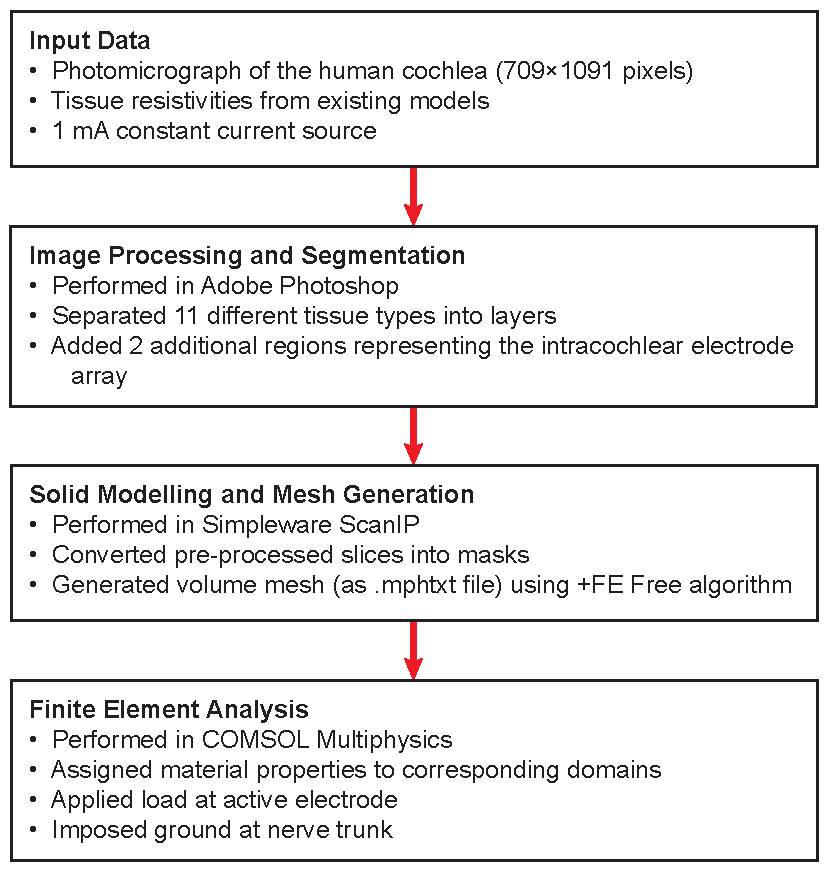
\includegraphics[width=11.8cm]{Methodology/workflow_poc}
	\caption[Workflow for the proof of concept model]{Workflow for the proof of
	concept model, indicating the programs used at each stage and the main tasks.}
	\label{fig:workflow_poc}
\end{figure}

\subsubsection{Imaging and Reconstruction}

The geometry of the model was based on a histological image of a section through
one turn of the human cochlea from Donkelaar and Kaga (see
Figure~\ref{fig:poc_histology})~\cite{donkelaar2011}. Image size was $ 709
\times 1091 $ pixels, and the relatively narrow field of view allowed the
various tissue types---including the membranes and blood vessels---to be easily
identified.

\begin{figure}
	\centering
	
	\begin{subfigure}[t]{0.35\textwidth}
        \centering
        \includegraphics[height=6.5cm]{Methodology/donkelaar_histo}
        \caption{ }
        \label{fig:poc_histology}
    \end{subfigure}%
    ~~~~
    \begin{subfigure}[t]{0.35\textwidth}
        \centering
        \includegraphics[height=6.5cm]{Methodology/donkelaar_segmented}
        \caption{ }
        \label{fig:poc_segmentation}
    \end{subfigure}%
    
	\caption[Image data for the proof of concept model]{Image data for the proof of
	concept model. (a) Photomicrograph of the human cochlea from Donkelaar and
	Kaga~\cite{donkelaar2011}; (b) the corresponding segmentation.}
	\label{fig:poc_model}
\end{figure}

The histological slice was pre-processed in Adobe Photoshop. Image contrast was
enhanced using the Auto Tone functionality to help distinguish the various
tissues of interest. Reissner's membrane required an additional gamma boost in
order to resolve the boundaries clearly. Eleven different tissue types (listed
under Table~\ref{table:poc_tissues}) were then manually segmented, with each
marked in its own layer using either the hard brush tool or the lasso tool with
feathering and anti-aliasing disabled to ensure accurate binarisation. Care was
taken to preserve the intricate shapes of the tissue structures, especially that
of the organ of Corti (note the tunnel of Corti and the tectorial membrane), the
double wall of the spiral lamina, and the modiolar bone. This fine anatomical
detail was important for ruling out simplifications in the model geometry as
sources of error.

\begin{table}
	\centering
	\sffamily
	
	\small
	\caption[Material properties for the proof of concept model]{Material
	properties for the proof of concept model. Resistivity values for this and the
	subsequent models were based on values from the literature per
	\S\ref{sect:material_properties} that were judged to be the most appropriate
	for the model.}
	\label{table:poc_tissues}
	
	\begin{tabularx}{0.4\textwidth}{X c}
		\toprule
		\textbf{Component}	& \textbf{Resistivity} \\
			& \textbf{($ \mathsf{\boldsymbol{\Omega}} \cdot $m)} \\
		\midrule
		\csvreader[late after line=\\]%
			{Methodology/poc_tissues.csv}%
			{1=\tissue,2=\resistivity}%
 			{\tissue & \resistivity}%
		\rule{0pt}{4ex}%
 		Silicone	& {$ \mathsf{1 \times 10^{7}} $} \\
		Platinum	& {$ \mathsf{1 \times 10^{-3}} $} \\
		\bottomrule
	\end{tabularx}
	
\end{table}

A Cochlear CI422 electrode array cross-section was added in the scala tympani at
a position and orientation that was consistent with images from a sectioned
implanted cochlea (courtesy Cochlear Limited). The final pre-processed image is
shown in Figure~\ref{fig:poc_segmentation}.

A stack of 22 copies of the pre-processed slice was then imported as a set of
backgrounds in Simpleware ScanIP. The images were slightly downsampled to
improve performance, and a mask for each material type was then created using
threshold segmentation. For some materials, such as perilymph and blood,
individual masks were created for separate structures to facilitate variation of
properties during subsequent analyses. The platinum contacts were only masked on
slices 5, 6, 11, 12, 17, and 18, thereby creating three evenly spaced electrode
pads with realistic separation distances. Smoothing and morphological filters
were applied to selected masks, taking care to patch any resultant gaps and
ensure continuity throughout the volume. The image stack was then upsampled in
the longitudinal direction to reduce the aspect ratio of the voxels in that
direction.

\subsubsection{Mesh Generation}

All masks were then used to construct a finite element mesh. Previous FEM and
BEM models have reported having difficulties meshing small structures like the
cochlear membranes~\cite{frijns1995,briaire2000mesh,hanekom2001,saba2012}. As
such, both of ScanIP's inbuilt meshing algorithms were tested.

The +FE Grid algorithm was quick and robust, and could easily handle the
complexity of the data. However, because it worked by starting with a finite
difference-style grid mesh based on the voxel size, the resultant volume mesh
was much denser than it needed to be (cf. Figure~\ref{fig:mesh_comparison}). The
time savings achieved through using this meshing algorithm would be easily
outweighed by the increase in solution time for subsequent simulations. Given
the likelihood of multiple testing scenarios during the analysis stages, a more
efficient mesh was sought.

The other algorithm, +FE Free, extended upon the grid mesh by converting it into
an unstructured tetrahedral mesh while largely respecting the domain boundaries.
The resultant meshes contain fewer nodes and fewer elements. This was not a
trivial task however, and the +FE Free algorithm took significantly longer than
+FE Grid to discretise a volume. The experience with the fine anatomical detail
in this model proved challenging, with the program often crashing unexpectedly
despite the headroom provided by the hardware setup (ScanIP reported a peak
working set of about 15 GB, which was well within the total RAM capacity of the
computer). A result was therefore not guaranteed, but tweaking the meshing
parameters over several iterations allowed the meshing algorithm to run to
completion and create a mesh of reasonable quality.

\subsection{Mesh Result}

The successful mesh is shown in Figure~\ref{fig:poc_mesh}. ScanIP took
approximately 1 hour and 40 minutes to generate this mesh. It consisted of
10,505,119 tetrahedral elements with 1,877,712 nodes. The average element
quality was 0.646, with most of the elements on the higher end of the scale as
indicated by a negatively skewed element quality histogram. ScanIP was able to
export the mesh in a number of different file formats. For the POC model, the
volume mesh was exported directly to COMSOL using an .mphtxt file.

\begin{figure}
	\centering
	
	% These images are from:
	%   B:\Models\2. Donkelaar-3D\4. COMSOL\Base\Donkelaar_25_SIP_base.mph
	%   which has been resaved with these updated camera settings
	\begin{subfigure}[t]{0.46\textwidth}
        \centering
        \includegraphics[height=6.4cm]{Methodology/poc_mesh_iso}
        \caption{}
        \label{fig:poc_mesh_iso}
    \end{subfigure}%
    ~~
    \begin{subfigure}[t]{0.52\textwidth}
        \centering
        \includegraphics[height=6.4cm]{Methodology/poc_mesh_zoom}
        \caption{}
        \label{fig:poc_mesh_zoom}
    \end{subfigure}%
    
	\caption[Volume mesh for the proof of concept model]{Volume mesh for the proof
	of concept model, generated using the +FE Free algorithm in ScanIP. (a) A
	global view showing the extruded direction; (b) a close up of the mesh around
	the organ of Corti, revealing the high element density required to discretise
	the fine structures.}
	\label{fig:poc_mesh}
\end{figure}

\subsection{Discussion}

The basic workflow established here was sufficient for converting an image of
the cochlea into a functional finite element model. However, the methodology
contained several limitations that could be improved in various ways.

Using a single histological image to build the model geometry allowed a high
level of detail to be incorporated within a relatively short timeframe, but the
true spiralling shape of the cochlea and the convoluted vascular trajectories
were not captured. Since the workflow could be adapted to any type of image
input, switching to a volumetric image stack would allow for a more realistic
reconstruction of the cochlear anatomy.

Building the electrode array using a set of additional masks was a quick way to
include a realistic array shape without the hassle of creating an extra model
via CAD. A similar process was followed by Girzon~\cite{girzon1987} and
Whiten~\cite{whiten2007}, though in the latter case the arrays were already part
of the image. Both of the inbuilt ScanIP meshing algorithms relied on the voxel
grid to create the mesh though, so there was potentially a degree of
discretisation error in play. The thickness of and longitudinal spacing between
electrode pads could not be controlled precisely with this method since they
were defined by the number of consecutive images containing or not containing
the electrode pad, respectively. It is therefore suggested that future models
define the electrode array using a CAD model.

Perhaps the most critical weakness of the POC method was the meshing algorithm.
Although it was able to produce a high quality mesh with conformal multi-part
surfaces, the coarseness parameter was not intuitively related to element size
and provided limited control over the mesh. Overriding these with manually set
parameters led to instability with the +FE Free algorithm that caused the
program to crash on multiple occasions. The need to follow a trial-and-error
process when adjusting these parameters and the high likelihood of failure were
not ideal. It also appeared that the algorithm could not handle high element
growth rates, leading to a higher than necessary mesh density. This is
particularly evident in Figure~\ref{fig:poc_mesh}, where the large volumes of
the scalae are filled with rather small elements. Given the direct impact of
element density on solution times and the other concerns raised above, a more
robust meshing workflow was sought for subsequent models.

% Determine a base case and consider parameters ceteris paribus.

%% ============================================================== Complex Models

\section{The Guinea Pig Model}
\label{sect:gp_model}

\subsection{Introduction}

Preliminary studies using the POC model~\cite{wong2012,inguva2015ner}
demonstrated that unrolled linear models of the cochlea were subject to several
limitations as a result of their simplified geometry. This is in line with
previous findings by Frijns~\cite{frijns1995} and Choi~\cite{choi2005}. As such,
a more sophisticated model featuring the true 3D geometry was desired.

Since the goals of the thesis required that the model possess a high level of
geometrical accuracy, multiple volumetric image stacks were sought. These
spanned a range of different imaging modalities, and after evaluating their
suitability for this project it was found that the most promising of these was a
scanning thin-sheet laser imaging microscopy (sTSLIM) image stack of the guinea
pig cochlea obtained by the Santi laboratory at the University of Minnesota.
Most importantly, all of the structural components of the cochlea could be
easily identified, including the different bone morphologies and the cochlear
vasculature. This unprecedented level of detail in the images allowed for a high
fidelity reconstruction, so this came to be the primary model for the
investigations in this thesis.

\subsection{Method}
\label{sect:method_gp}

\textit{This section is based on the paper by Wong~\etal~\cite{wong2016}, which
has been published in IEEE Transactions on Biomedical Engineering.}

A modular workflow based on that used by Tran~\etal{}~\cite{tran2015} was
adopted in order to overcome the segmentation and meshing challenges typically
encountered in electroanatomical modeling~\cite{briaire2000mesh}. The main steps
are summarised in Figure~\ref{fig:workflow_gp}. The best features of several
programs were selectively combined to create a more accurate model than would
otherwise have been possible.

\begin{figure}
	\centering
	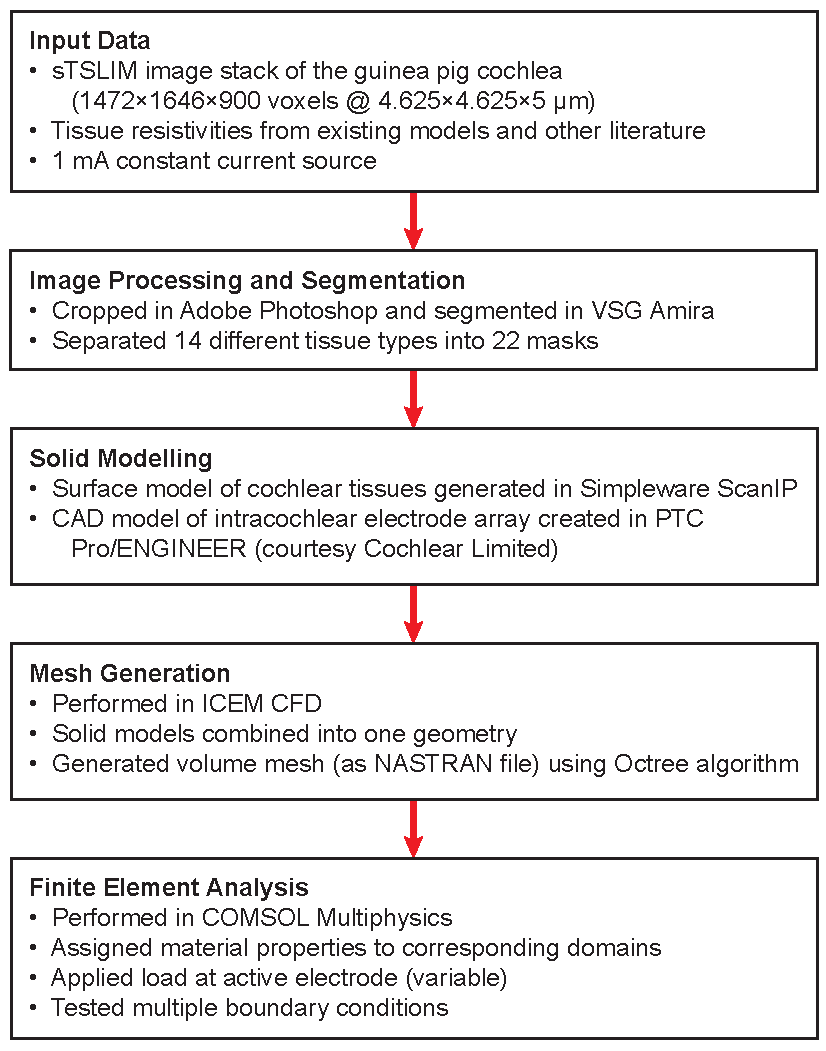
\includegraphics[width=11.8cm]{Methodology/workflow_gp}
	\caption[Workflow for the guinea pig model]{Workflow for the guinea pig
	model. It was extended from that of the POC model to provide more flexibility
	and control, and was able to overcome the problems encountered when meshing
	with ScanIP.}
	\label{fig:workflow_gp}
\end{figure}

\subsubsection{Imaging and Reconstruction}
\label{sect:sTSLIM_imaging}

A high resolution ($ 4.625 \times 4.625 \times 5~\upmu$m voxel size) sTSLIM
image stack of the guinea pig cochlea was used as the geometrical basis for the
model (see Figure~\ref{fig:gp_tslim}). This technique combines the high
resolution and clarity of optical microscopy with the non-destructive nature of
computed tomography (CT) and magnetic resonance imaging (MRI), making it ideal
for capturing fine anatomical details~\cite{santi2011,buytaert2013}. The cochlea
was explanted from a healthy guinea pig of unknown age, with no visible scar
tissue and only minor neuronal degeneration at the basal end. Both soft and hard
tissues were identifiable, and the images were predominantly free of absorption
artifacts.

\begin{figure}[t]
	\centering
	
	\begin{subfigure}[t]{0.5\textwidth}
        \centering
        \includegraphics[height=9cm]{Methodology/segmentation_tslim}
        \caption{}
        \label{fig:gp_tslim}
    \end{subfigure}%
    \begin{subfigure}[t]{0.5\textwidth}
        \centering
        \includegraphics[height=9cm]{Methodology/segmentation_masks}
        \caption{}
        \label{fig:gp_masks}
    \end{subfigure}%
    
	\caption[Segmentation of the sTSLIM images]{Segmentation of the sTSLIM images.
	(a) A mid-modiolar image from the sTSLIM stack; note the high resolution and
	clarity in both the soft and hard tissues. (b) 14 tissue types were
	identified in the voxel space; these were separated into 22 different masks to
	aid with visualisation and modelling. (Copyright \textcopyright{} 2015, IEEE.)}
	\label{fig:gp_segmentation}
\end{figure}

Fourteen different tissue types were then identified and segmented. These are
illustrated in Figure~\ref{fig:gp_masks} and listed in
Table~\ref{table:gp_domains}. Segmentation was initially performed in Photoshop
as per the POC model, but it was soon discovered that this method was not ideal
because alignment between slices could not be guaranteed. It was also difficult
to see the outcomes of the segmentation. The open source program
\href{http://www.slicer.org/}{3D Slicer} was able to provide a 3D visualisation
of the segmented stack, but the cumbersome nature of using multiple programs
during this stage was a drag on efficiency.

Consequently, a semi-manual process was adopted using Amira v5.4.2
(Visualization Sciences Group, Burlington MA, USA). The main advantage of this
program was that it provided a 3D view of the segmented voxel space that was
updated in real-time. For each tissue, a region in one image was selected with
the aid of luminance thresholds. The selection was then smoothed, and the
process repeated on the adjacent slice. If there was minimal variation in shape
between successive slices, the next selection would be made several slices away
and the volume in between was selected via interpolation. This preserved the
organic appearance of the tissues while reducing the amount of data to be
processed. Bone was separated by morphology as this was found to be an important
factor for model accuracy and could actually be differentiated in the sTSLIM
scans~\cite{wong2013mb}. Nerve, perilymph, endolymph, and blood were also
categorised by anatomical structure to aid with visualisation (see
Table~\ref{table:gp_domains}). The thin membranes between the scala vestibuli
and the vestibular complex were excluded in this reconstruction, as per other
models. Finally, some additional smoothing was applied, and any remaining voxel
fragments were allocated to adjacent masks using the island removal tool to
ensure continuity throughout the volume in preparation for mesh generation.

\begin{table}
	\centering
	\sffamily
	\small
	\caption[Material domains in the guinea pig model]{Material domains in the
	guinea pig model.}
	\label{table:gp_domains}
	
	\begin{tabularx}{0.77\textwidth}{X c c c}
		\toprule
		\textbf{Component}	& \textbf{~Resistivity~} &
				\multicolumn{2}{c}{\textbf{Element size limits (mm)}} \\
			& \textbf{($ \mathsf{\boldsymbol{\Omega}} \cdot $m)}
				& \textbf{~~Minimum~~} & \textbf{Maximum} \\
		\midrule
		\csvreader[late after line=\\]%
			{Methodology/gp_tissues.csv}%
			{1=\tissue,2=\resistivity,3=\min,4=\max}%
 			{\tissue & \resistivity & \min & \max}%
		\rule{0pt}{4ex}%
	    Silicone	& {$ \mathsf{1 \times 10^{7}} $} 	& 0.0625	& 0.0625 \\
		Platinum	& {$ \mathsf{1.06 \times 10^{-7}} $}	& 0.03125	& 0.03125 \\
		\bottomrule
	\end{tabularx}
		
\end{table}

The segmented domains were exported into ScanIP, and masks were created for each
tissue by using the pre-segmented data mask generator on the segmented image
stack. A surface model was then generated from the binarised masks in a
stereolithography (STL) format. The pre-smoothing and part change options were
enabled to avoid jagged surfaces, and decimation was disabled to ensure
conformity between adjacent components. The resulting reconstruction is shown in
Figure~\ref{fig:gp_model}.

\begin{figure}
	\centering
	
	\begin{subfigure}[t]{\textwidth}
        \centering
        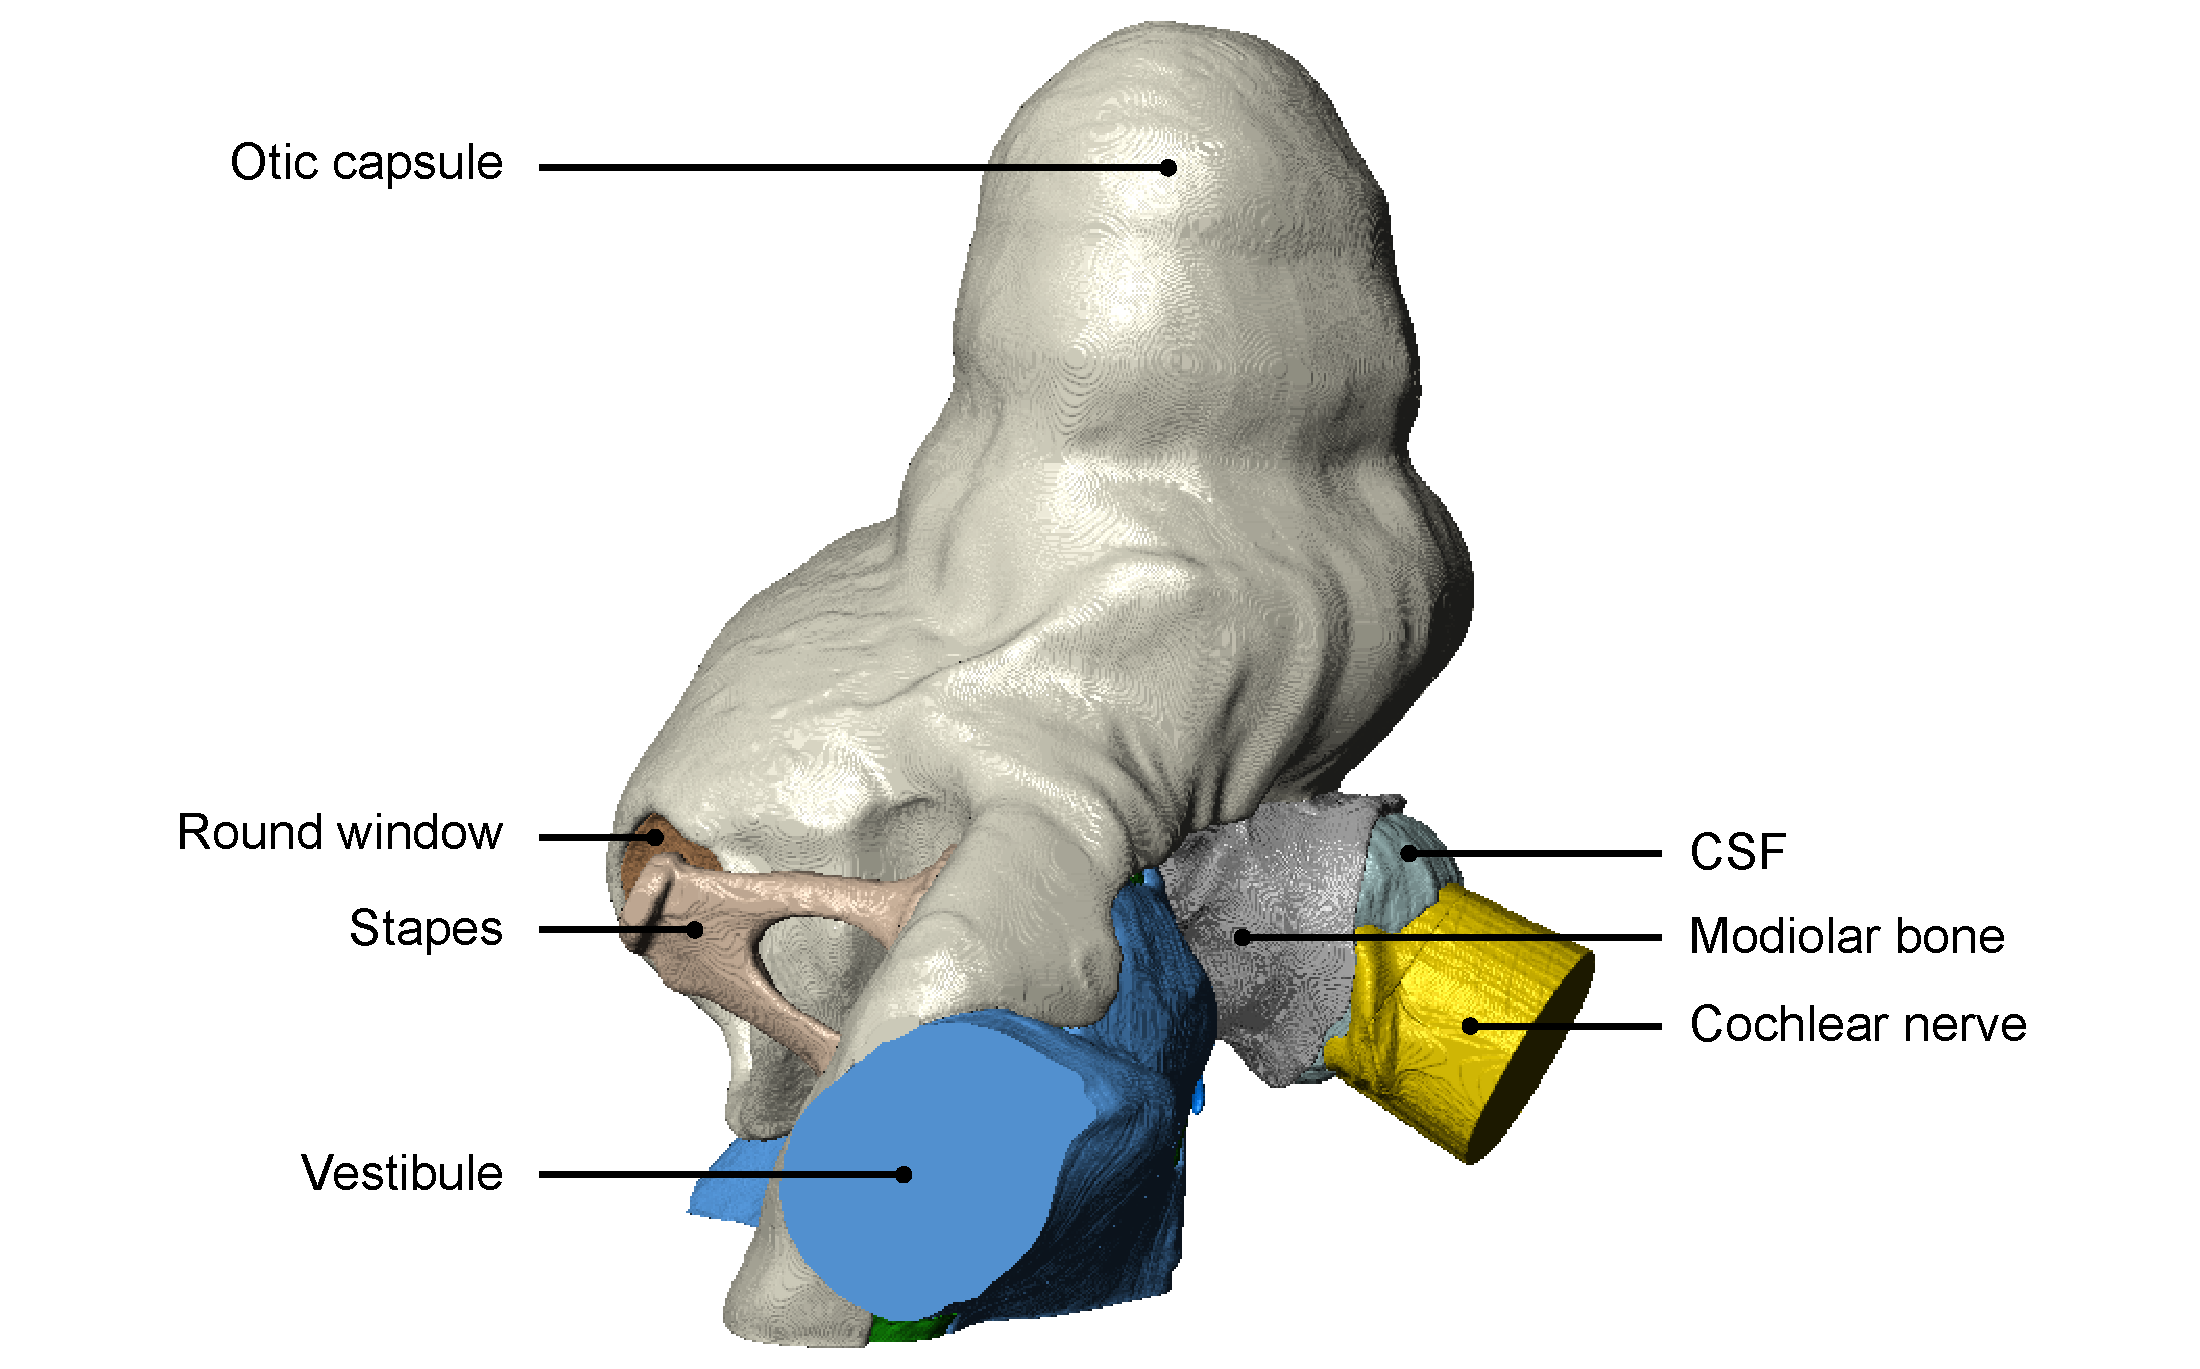
\includegraphics[height=8.5cm]{Methodology/cochlea_labelled_opaq}
        \caption{}
        \label{fig:gp_outer}
    \end{subfigure}\\%
    \vspace{1em}%
	\begin{subfigure}[t]{\textwidth}
        \centering
        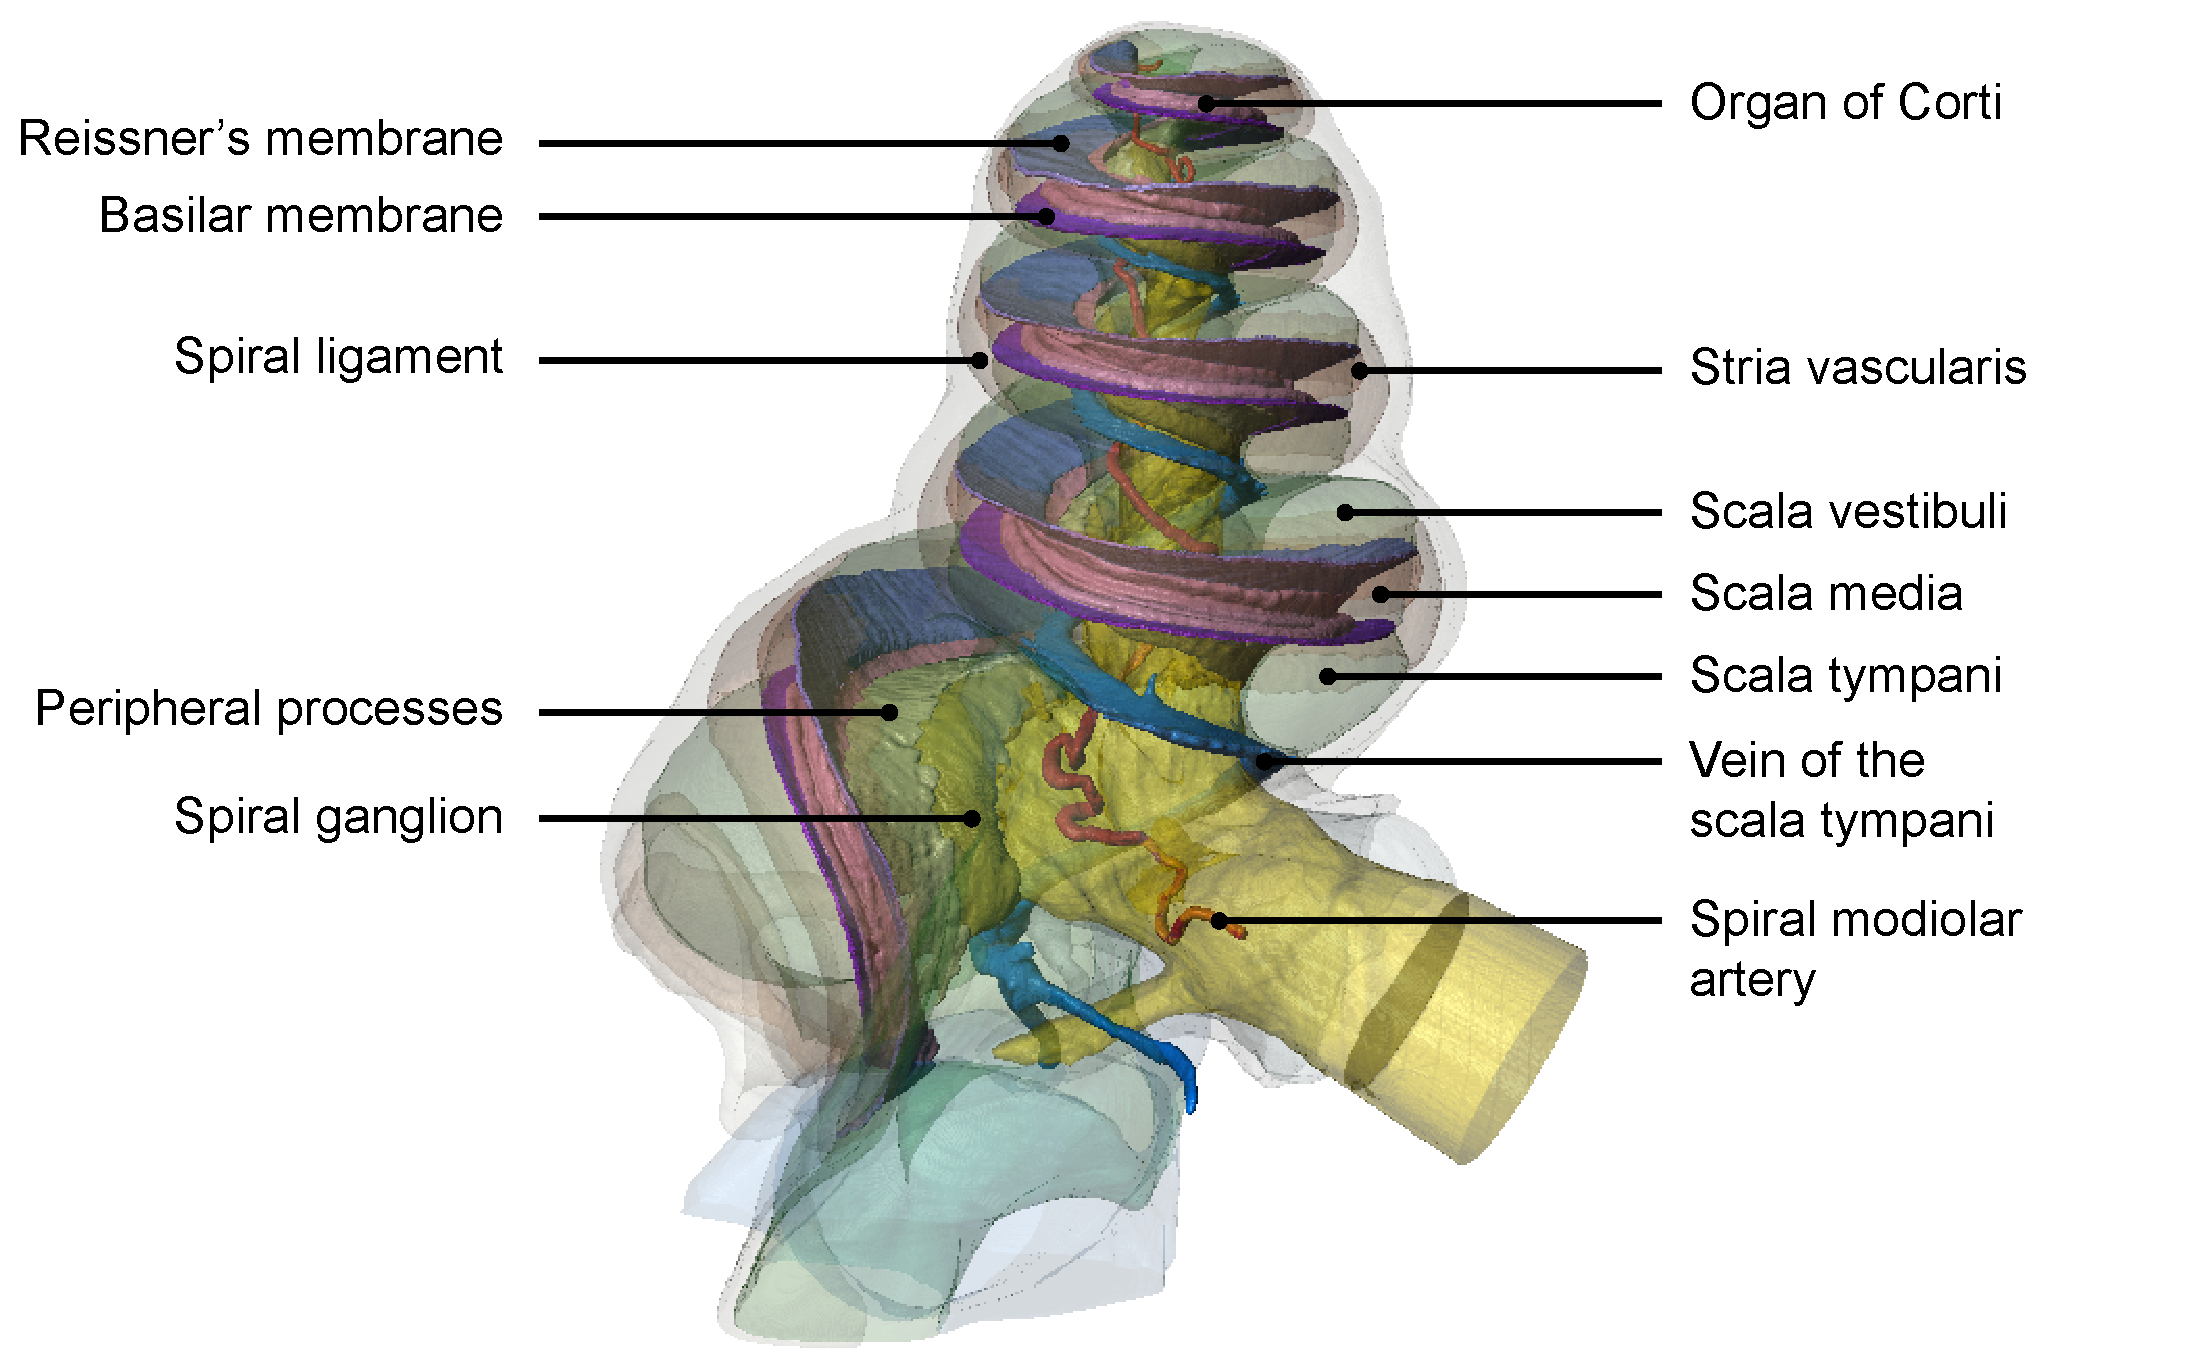
\includegraphics[height=8.5cm]{Methodology/cochlea_labelled_trans}
        \caption{}
        \label{fig:gp_inner}
    \end{subfigure}%
    
	\caption[Surface reconstruction of the guinea pig model]{Surface reconstruction
	of the guinea pig model. (a) The cochlea is surrounded by the hard outer bone
	of the otic capsule; (b) removing the bone layers reveals the scalae, soft
	tissues, neural structures, and blood vessels deeper in the cochlea. (Copyright
	\textcopyright{} 2015, IEEE.)}
	\label{fig:gp_model}
\end{figure}

\subsubsection{Mesh Generation}
\label{sect:gp_mesh_gen}

The STL files were imported into ICEM CFD v15.0 (ANSYS Incorporated, Canonsburg
PA, USA) for volume meshing. A CAD model resembling the Cochlear Limited
Hybrid-L8 (HL8) electrode array was inserted through the round window and into
the scala tympani in a mid-scala position (see Figure~\ref{fig:hl8_insertion}).
The electrodes along this array were numbered from E1 at the basal end to E8 at
the apical end. Insertion depth was just over 6 mm, corresponding to an
insertion angle of about 380 degrees at E8. A build topology operation was
performed to ensure that the mesh respected the smooth curves of the array
model.

\begin{figure}
	\centering
	\includegraphics[width=7.5cm]{Methodology/hl8_insertion}
	\caption[Virtual insertion of the HL8 array into the scala tympani]{Virtual
	insertion of the HL8 array into the scala tympani.}
	\label{fig:hl8_insertion}
\end{figure}

Since orthogonal surfaces artificially draw current toward the center of each
face~\cite{wong2013ciap}, the virtually implanted cochlea was embedded in a
sphere of radius 5~mm to facilitate the application of boundary conditions. This
size was found to be sufficiently large for replicating far-field
effects~\cite{wong2013ciap}. Unlike the human cochlea, which is encased within
the temporal bone, the guinea pig cochlea protrudes into the tympanic
bulla~\cite{cooper1975}, so injected current must flow towards the temporal
bone. The surrounding sphere was therefore angled such that one hemisphere
extended into the tympanic bulla and the other into the surrounding temporal
bone (hereafter referred to as the ``temporal bone surface''; see dark grey
hemisphere in Figure~\ref{fig:gp_mesh_all}), matching the bone boundary in the
scans. A second concentric sphere of radius 8~mm was subsequently added to
create an additional surrounding domain. This was used to define an infinite
element domain for the boundary condition studies.

Element sizes for each component were established to balance node count against
geometrical accuracy. A volume mesh was then generated using ICEM CFD's top-down
Octree algorithm. Finally, any small element islands resulting from the process
were assigned to an adjacent domain to simplify the subsequent FEA steps. The
final mesh is shown in Figure~\ref{fig:gp_mesh}.

\begin{figure}
	\centering
	
	\begin{subfigure}[t]{0.5\textwidth}
        \centering
        \includegraphics[height=7.5cm]{Methodology/gp_mesh_solid}
        \caption{}
        \label{fig:gp_mesh_solid}
    \end{subfigure}%
    %
    \begin{subfigure}[t]{0.5\textwidth}
        \centering
        \includegraphics[height=7.5cm]{Methodology/gp_mesh_lines}
        \caption{}
        \label{fig:gp_mesh_lines}
    \end{subfigure}\\%
    \vspace{1em}%
    \begin{subfigure}[t]{\textwidth}
        \centering
        \includegraphics[height=8cm]{Methodology/gp_mesh_all}
        \caption{}
        \label{fig:gp_mesh_all}
    \end{subfigure}%
    
    \caption[Volume mesh of the guinea pig model]{Volume mesh of the guinea pig
    model. (a) Solid element view of the guinea pig cochlea. (b) Outline
    view of the mesh, revealing the inner structures. (c) The cochlea shown
    within the surrounding bone spheres.}
	\label{fig:gp_mesh}
\end{figure}

\subsubsection{Estimating Neuronal Trajectories}

In order to gain some insight into the simulated neural response, the activating
function (AF, per Equation~\ref{eqn:af}) was calculated because it signifies the
degree to which the underlying electrophysiological requirements for neural
firing are met. This required finding the second derivative of the voltage
scalar field \emph{along the neuron}. Since the geometry in this model was based
on an image stack, there was no simple equation-based method for fitting nerve
fibre trajectories within the neural tissue~\cite{escude2006}. Computational
methods for extracting the vector field of the fibre orientations from the
volumetric images (like those used by Bishop in cardiac
tissue~\cite{bishop2010}) were considered, but these are difficult to implement
and were not guaranteed to work with the images that had been acquired.
Therefore, a semi-manual spline interpolation method was used for estimating the
neuronal trajectories.

For this model, nerve fibres covering approximately the first 570 degrees of the
cochlea were modelled in MATLAB (The Mathworks Inc., Natick MA, USA). This was
sufficient for covering the main areas of excitation for the observed insertion
depth of the HL8 array. Each fibre was assumed to run through a number of key
locations: from the tip of the peripheral processes, through the centre of the
spiral ganglion, then joining the auditory nerve trunk in the modiolus. This was
similar to existing modelling studies, such as that shown in Figure~2b by
Kalkman~\etal{}~\cite{kalkman2014}. The tonotopic organisation of the fibres was
preserved, i.e. the more basal axons followed a path near the circumference of
the nerve trunk, while progressively more apical axons spiralled inwards towards
the core of the trunk.

Nodes of Ranvier were positioned along each neuron at fixed intervals from the
point in Rosenthal's canal. Internodal spacing was chosen to resemble that used
in the GSEF neural model~\cite{frijns1995}: 175~$ \upmu $m along the peripheral
process and 300~$ \upmu $m along the axon. The node points were determined
using the
\href{http://in.mathworks.com/matlabcentral/fileexchange/34874-interparc}{\emph{interparc}}
and
\href{http://au.mathworks.com/matlabcentral/fileexchange/34871-arclength}{\emph{arclength}}
functions published by John D'Errico on the MATLAB File Exchange (licences
shown in Appendix~\ref{appendix:licences}).

The final interpolated fibre trajectories are shown in
Figure~\ref{fig:fibre_trajectories}. Using these neuronal trajectories, the AF
was then computed for each set of adjacent nodal triads along 100 fibers spaced
equally along the cochlear spiral.

\begin{figure}
	\centering
	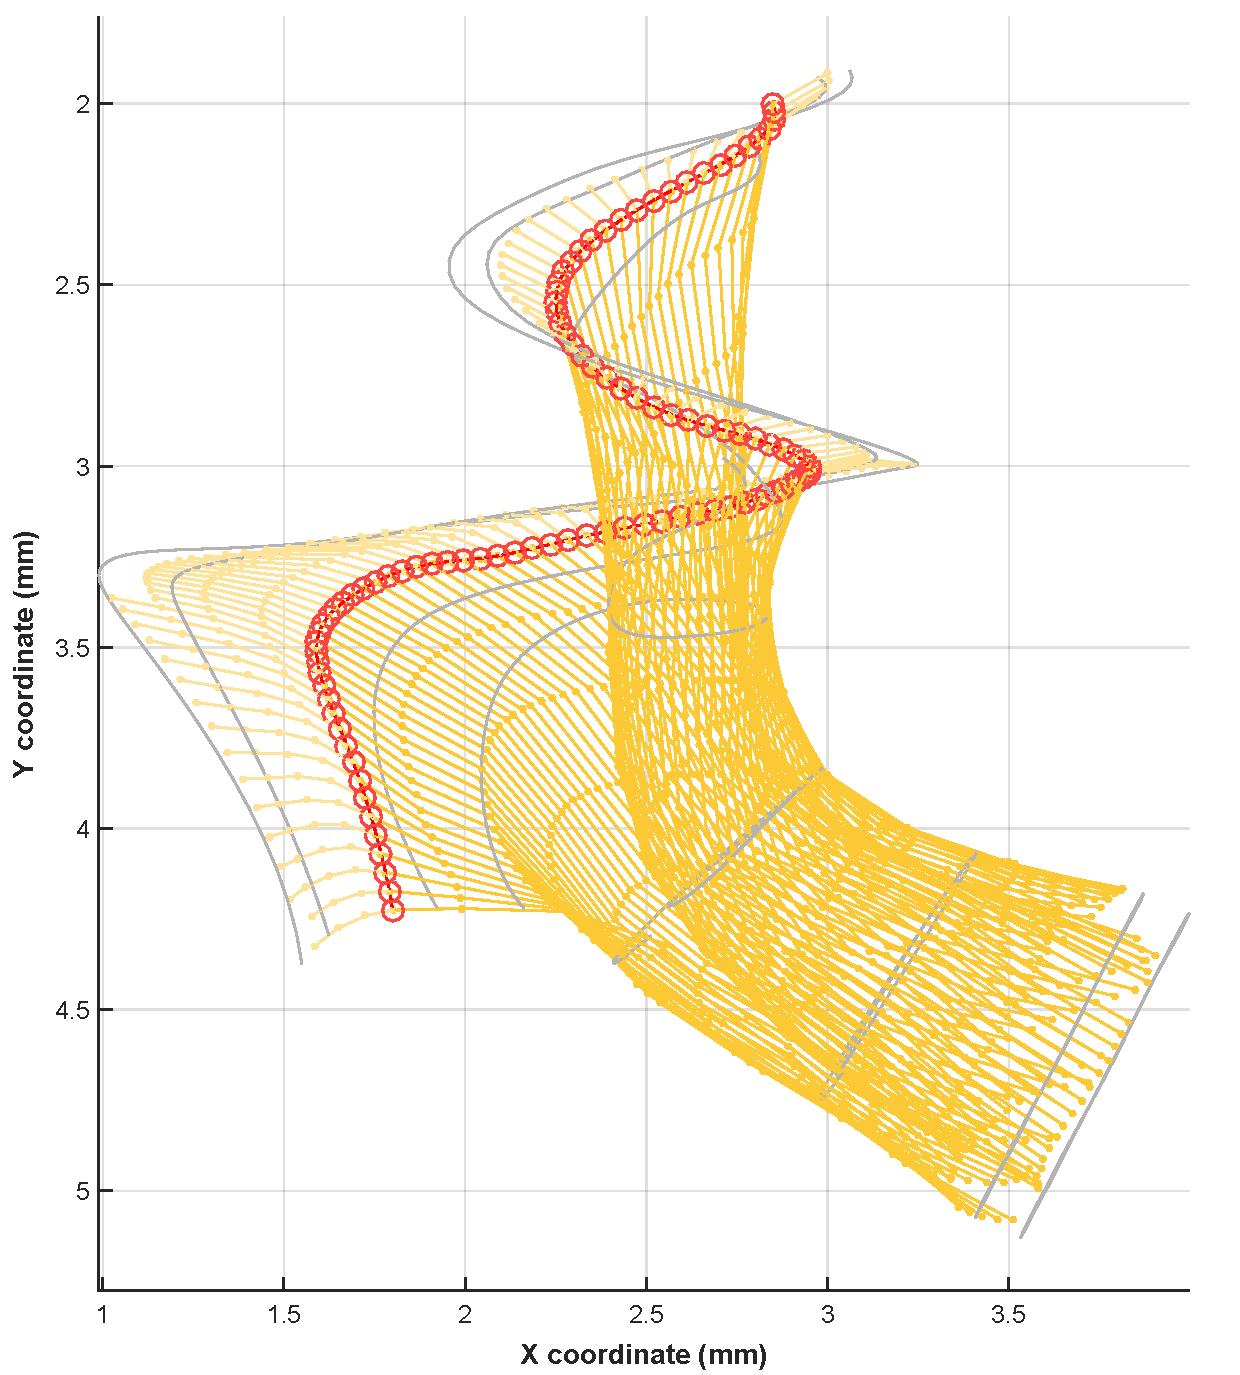
\includegraphics[width=\textwidth]{Appendix/fibres-100}
	\caption[XY view of nerve fibre trajectories]{XY view of nerve fibre
	trajectories, estimated using MATLAB. Guide splines (grey) were determined
	from manually selected key points along the auditory nerve from the distal
	end of the peripheral process, through the centre of the spiral ganglion
	(marked by red circles), to the end of the modelled nerve trunk. Nodes of
	Ranvier were estimated along each fibre, and the electric potential at those
	points was used to calculate the activating function.}
	\label{fig:fibre_trajectories}
\end{figure}

% \subsubsection{Model Outputs}

% Derived values. Expression used for flux through nerve:
% 	nx*ec.Jx+ny*ec.Jy+nz*ec.Jz. 
% May need negative, check direction of normal to surface.

\subsection{Mesh Result}

ScanIP took approximately 1 hour and 30 minutes to generate the surfaces, while
ICEM CFD took another 1 hour and 30 minutes to generate the volume mesh. The
base case volume mesh consisted of 4,684,028 tetrahedral elements with 790,653
nodes. A handful of small, spurious element islands were formed due to the way
the Octree algorithm works, so some additional time was required to identify the
tissues to which these elements belonged and merge them together. Following
this, the mesh was successfully exported using the NASTRAN file format.

The volume mesh created here possessed a more appropriate balance between
element size growth rate and quality compared with the POC model. Despite
covering a much larger region of interest, it had fewer elements and a higher
average element quality of 0.712. On the downside, boundaries where three or
more tissues touched did not perfectly conform to the smooth input surfaces,
again due to the top-down approach of the Octree algorithm. A close up view of
the spiral ligament in Figure~\ref{fig:gp_mesh_jaggies} provides some idea of
the extent of this issue. The bulk of the tissue volume did not suffer from this
problem.

\begin{figure}
	\centering
	\includegraphics[width=8cm]{Methodology/gp_mesh_jaggies}
	\caption[Jagged boundaries in the volume mesh]{Jagged boundaries in the volume
	mesh due to the top-down approach of ICEM CFD. This close up shows part of the
	spiral ligament, which is routinely interfacing with multiple tissues.}
	\label{fig:gp_mesh_jaggies}
\end{figure}

% Boundary condition sensitivity (including infinite elements), Blood vessel
% sensitivity, electrode positioning sensitivity, convergence test, sensitivity to
% bone and spiral ligament resistivities

\subsection{Discussion}

The experience of this project mirrors that of
Briaire~\etal{}~\cite{briaire2000mesh} in that discretising the volume was the
most difficult step. A similar conclusion was also reached by
Saba~\cite[Appendix G]{saba2012} and the Hanekom group [personal communication],
both of whom struggled to mesh the organic shape of the cochlea in COMSOL. This
is presumably why some VCMs of the cochlea used such simplified
geometries~\cite{finley1990,tognola2007}.

The high resolution of the sTSLIM scans was a double-edged sword. It allowed for
much of the fine anatomical detail to be seen and incorporated, making for a
more realistic model. However, the presence of this additional detail clearly
contributed to the meshing difficulties. ScanIP was unable to directly generate
a working volume mesh due to the complexity of the surfaces, and ICEM CFD would
sometimes crash while importing the STL files (though the reason for this was
less clear and may be due to a software bug). Many of the cochlear tissues are
also quite thin, which meant that a very fine mesh was required to maintain a
reasonable element quality. The ability of the Octree algorithm to conform to
the surfaces and transition from very small elements to significantly larger
ones in the bulk regions of the scalae and surrounding bone are a testament to
its robustness. A hexahedral mesh would have been preferred over the tetrahedral
mesh for accuracy, but attempts to create such a mesh in ICEM CFD failed to
produce a result. The Octree mesh did exhibit some discretisation error at some
of the interfaces, but this is expected to have minimal impact on the results of
interest because the number of affected elements is small relative to the
overall volume and the measurements are taken some distance away from these
boundaries.

In terms of sourcing appropriate material properties, the values are typically
assumed to be similar between humans and guinea pigs. The main exception is that
of bone, for which more appropriate data was available: here, the resistivities
for guinea pig bone were taken from the measurements of
Suesserman~\cite{suesserman1992}. Like other VCMs of the cochlea though, the
reliability of the tissue resistivities is a potential weakness due to the low
number of independent data sources. A sensitivity analysis was therefore
performed as part of the validation study in Chapter~\ref{sect:validation}.

Sources of error for the neuronal component were threefold. Firstly, the
trajectories could be further improved: nerve fibre density is not uniform
throughout the cochlear turns~\cite{bredberg1965,spoendlin1985}, and the
bunching of peripheral processes and the curved trajectory towards the
apex~\cite{wright2005} was not reflected in the model. Secondly, the internodal
spacing used in the GSEF model is based on measurements in the cat by
Liberman~\cite{liberman1984}. These may not be suitable for the guinea pig. The
additional simplification of constant length intervals would also have a bearing
on the AF results. It is worth noting at this point that neural degeneration and
demyelination can occur with deafness, altering current distribution and neural
excitation predictions respectively near the damaged regions. Since the guinea
pig model was compared with acute experimental data from implanted but otherwise
healthy animals in this thesis, these factors were not incorporated. Finally,
the use of the AF instead of a more complete model of neural kinetics limits the
current iteration of this model in that thresholds cannot be predicted. Given
the focus of this thesis on the physics that underpin volume conduction in the
cochlea and the inconsistencies of existing excitation models, it was decided
that the AF would suffice for demonstrating the likelihood of excitation and
that neural kinetics would best be left to future extensions of this project.
For reference though, the early guinea pig models by Frijns~\etal{} predicted
excitation thresholds for bipolar configurations at a stimulus current of around
1~mA~\cite{frijns2000, briaire2000field}, while \invivo{} measurements by
Huang~\etal{} found thresholds of around 0.35~mA~\cite{huang1999reduction}.
Threshold currents for monopolar configurations are expected to be lower than
these values, as discussed in \S\ref{sect:electrode_configs}.

% The activation function is determined using the discrete form to give an
% indicator of the likelihood of neural excitation. Note that it holds in the
% linear regime of the neural membrane (below threshold), but does not accurately
% represent the situation close to threshold due to non-linear behaviour. Neural
% kinetic models are required for this. However should be suitable for the
% purposes of showing differences.

Despite these limitations, the model should be able to elucidate insightful
spatial trends along the cochlear spiral.

\section{The Human Model}
\label{sect:human_model}

\subsection{Introduction}

The third model that was made for this project was a subject-specific human
cochlea. Its main aims were to test the feasibility of the methodology on a
different image dataset, demonstrate the differences in geometry between human
and guinea pig cochleae, and be incorporated with a detailed model of the human
head from a parallel project~\cite{tran2015} for a multiscale simulation. The
initial development of this human cochlear model formed the basis for a second
undergraduate honours thesis in 2014. The following section describes some of
the work performed as part of that project as well as the additional work to
create a more accurate iteration.

\subsection{Method}

The workflow used for the human model was essentially the same as that used for
the guinea pig model (Figure~\ref{fig:workflow_gp}), but with some of the
segmentation performed algorithmically in ScanIP. Learning efficiencies obtained
while working with the earlier models were put into practice during this
implementation, speeding up model creation.

\subsubsection{Imaging and Reconstruction}

The human model was based on a microCT dataset of a preserved human temporal
bone containing a previously implanted cochlea. Preparation and scanning of the
specimen were performed by Ian Curthoys from the School of Psychology and
Christopher Wong from the Australian Centre for Microscopy and Microanalysis
(ACMM), both at the University of Sydney. The images obtained (see
Figure~\ref{fig:human_microCT}) were both clean and detailed, with a field of
view that was wide enough to include the semicircular canals. The $ 1479 \times
1501 \times 1114 $ voxel space had an isotropic resolution of 27~$ \upmu $m, so
the microCT scans were not as detailed as the sTSLIM images of the guinea pig
but still provided sufficient resolution to construct a reasonably accurate
model.

\begin{figure}
	\centering
	\includegraphics[width=8.5cm]{Methodology/Gibson_axial_0687}
	\caption[MicroCT image of the human temporal bone]{MicroCT image of the human
	temporal bone.}
	\label{fig:human_microCT}
\end{figure}

The main improvements of this model over the preliminary iteration were the
inclusion of additional tissue masks (for the otic capsule, modiolar bone, CSF,
and vestibular nerves) and refinement of existing masks, most notably those for
the facial nerve and the spiral ganglion. A complete list of segmented tissues
is provided in Table~\ref{table:human_domains}. For most of these tissues,
segmentation was performed semi-manually as per the guinea pig model. A greater
focus was placed on using the interpolation functionality of Amira as this
enabled the organic smoothness of the anatomy to be preserved. The vestibular
structures of the inner ear were included in this model since they were within
the field of view of the scans, and there is evidence to suggest that the
largest fraction of injected current leaves the cochlea via the nearby basal
end~\cite{vonbekesy1951,vanpoucke2004identification}.

\begin{table}
	\centering
	\sffamily
	\small
	\caption[Material domains in the human model]{Material domains in the
	human model.}
	\label{table:human_domains}
        
	\begin{tabularx}{0.72\textwidth}{X c c c}
		\toprule
		\textbf{Component}	& \textbf{~Resistivity~} &
				\multicolumn{2}{c}{\textbf{Element size limits (mm)}} \\
			& \textbf{($ \mathsf{\boldsymbol{\Omega}} \cdot $m)}
				& \textbf{~~Minimum~~} & \textbf{Maximum} \\
		\midrule
		\csvreader[late after line=\\]%
			{Methodology/human_tissues.csv}%
			{1=\tissue,2=\resistivity,3=\min,4=\max}%
 			{\tissue & \resistivity & \min & \max}%
 		\rule{0pt}{4ex}%
 		Silicone	& {$ \mathsf{1 \times 10^{7}} $} 	& 0.0625	& 0.0625 \\
		Platinum	& {$ \mathsf{1.06 \times 10^{-7}} $}	& 0.03125	& 0.0625 \\
		\bottomrule
	\end{tabularx}

\end{table}

The otic capsule around both the cochlea and the semicircular canals required
special treatment. A preliminary outline was created by dilating a mask of the
corresponding fluid chambers in ScanIP into the regions occupied by the dense
bone immediately surrounding the inner ear (as depicted by the lack of voids in
the microCT data). This mask was then reimported into Amira for further
refinement and integration with the other segmented tissues (see
Figure~\ref{fig:human_segmentation}). The otic capsule mask slightly exceeded
the scanned specimen in the region of the semicircular canals because the
lateral aspect of one of the canals was cut into slightly during the original
extraction of the temporal bone sample.

\begin{figure}[p]
	\centering
	\includegraphics[height=7cm]{Methodology/human_segmentation}
	\caption[Segmentation of the microCT images]{Segmentation of the microCT
	images. Superfluous regions were cropped from the original scans to reduce
	RAM usage.}
	\label{fig:human_segmentation}
\end{figure}

\begin{figure}[p]
	\centering
	\includegraphics[height=7cm]{Methodology/Gibson_HM_PhD_v1}
	\caption[Surface reconstruction of the human cochlear model]{Surface
	reconstruction of the human cochlear model.}
	\label{fig:human_model_surface}
\end{figure}

After all tissue masks were finalised, the pre-processed image stack was again
imported into ScanIP for surface reconstruction, resulting in the surface
model shown in Figure~\ref{fig:human_model_surface}.

\subsubsection{Mesh Generation}

As per the guinea pig model, the human model was discretised using ICEM CFD. The
surfaces generated in ScanIP were imported into ICEM as faceted STL geometries,
along with a CAD model of an intracochlear electrode array with 22 contacts,
which was inserted along a mid-scalar path. A build topology operation was
performed on the array to ensure that node placement conformed to the smooth
edges defined in the CAD model, as per the guinea pig model.

Various meshing parameters were set up in a similar manner to that used
previously. Maximum and minimum element sizes that provided a good balance
between geometrical accuracy and node count were determined. The final element
size limits used for this model are listed in Table~\ref{table:human_domains}.
The Octree algorithm was used once again for the actual discretisation
step, and the successful mesh was exported as a NASTRAN file.

\subsection{Mesh Result}

The final volume mesh for the human cochlear model is shown in
Figure~\ref{fig:human_model_mesh}. Due to its relative simplicity, it only took
about 15 minutes to compute. It consisted of 1,877,793 tetrahedral elements and
318,236 nodes. The average element quality was 0.712, similar to that of the
guinea pig mesh.

\begin{figure}[t]
	\centering
	\includegraphics[width=10cm]{Methodology/hm_mesh}
	\caption[Volume mesh of the human cochlear model]{Volume mesh of the human
	cochlear model. The size of the surrounding sphere was deliberately chosen
	such that the ends of N VII and N VIII protruded slightly. The
	Octree algorithm would automatically identify the intersecting surface,
	facilitating the application of traditional boundary conditions.}
	\label{fig:human_model_mesh}
\end{figure}

\subsection{Discussion}

The robustness of the methodology was clearly demonstrated by the successful
creation of another complex mesh. Given that it was a second attempt at
implementing the workflow, learning efficiencies significantly sped up the model
creation process. Subsequent reconstructions can be expected to be even faster,
perhaps even reaching a six week turnaround between scanning and the finalised
reconstruction.

Another factor that reduced the required modelling time was the use of a lower
resolution dataset. The smaller voxel space of the microCT data meant that less
data needed to be processed to create the human model than was required for the
sTSLIM data used for the guinea pig model. However, it also meant that some of
the finer anatomical details were not visible and thus could not be incorporated
into the model. The most notable omissions were the soft tissue structures,
which were difficult to identify given the larger voxel size and the scanning
technique used. The cochlear partition needed to be modelled as a single part
because it was impossible to distinguish the spiral lamina, peripheral
processes, organ of Corti, and basilar membrane, and the inability to resolve
Reissner's membrane meant that the scala media could not be modelled. The
cochlear blood vessels could not be segmented for similar reasons.

One way this might be offset in future studies is to divide the volume into
smaller regions, scan each of them individually, and finally realign them to
produce a larger voxel space. This would introduce a number of extra challenges,
such as correct realignment of the subsections, and could be cost prohibitive,
but would yield a much higher resolution reconstruction. Better image data may
also be obtained as sTSLIM techniques for human specimens become more refined.
If such paths were pursued, the additional computational cost required at each
stage of the pipeline would also need to be taken into account to ensure
feasibility. Additional pre-processing steps, such as adding an anisotropic
diffusion filter to the image data prior to
segmentation~\cite{poznyakovskiy2008}, could make the reconstruction easier to
manage in that case, but care would be required to ensure that the anatomical
structures do not become too distorted.

Looking further ahead, the main challenge left to address in the workflow is
improving the reliability of the discretisation step. Noticeably fewer element
islands were produced in the human model, likely a by-product of the simpler
segmentation, but they could not be completely and consistently eliminated. This
meant that manual inspection of the mesh was always required, a step which was
extremely time-consuming because the complexity of the surfaces caused the
graphics subsystem to lag during all interactions with the user interface.
Alternative meshing programs may yield better results in this respect.

\section{Chapter Summary}

A robust modelling workflow was established by combining the best aspects of
several different programs. The various types of data required as input to the
workflow were each critically considered. In the end, three different finite
element models of the cochlea were produced: (i) a simply extruded proof of
concept model, which was used to evaluate the basic workflow requirements, (ii)
a highly detailed guinea pig model that became the primary model for subsequent
investigations, and (iii) a human model, for comparison with the guinea pig
model and integration with a human whole head model. High quality meshes were
produced for all three models. These were imported into COMSOL Multiphysics for
running further analyses. The insights gained from these studies are documented
in the following chapters and aim to shed some light on the issues raised under
\S\ref{sect:research_questions}.
